\documentclass{article}
\usepackage[utf8]{inputenc}
\usepackage{graphicx}
\usepackage[
backend=biber,
style=authoryear,
citestyle=authoryear
]{biblatex}
\renewcommand*{\bibfont}{\small}
\usepackage[normalem]{ulem}
\usepackage{fancyhdr}
\usepackage{multicol}
\usepackage[hidelinks]{hyperref}
 
\pagestyle{fancy}
\fancyhf{}
\rhead{The Effect of News Framing}
\lhead{Berk}
\cfoot{\thepage}

\useunder{\uline}{\ul}{}

\addbibresource{PhD-Proposal.bib}


\usepackage{xcolor}

\title{The Causal Effect of News Framing on Opinion Formation}
\author{Nicolai Berk\footnote{Doctoral Candidate, Dynamics Doctoral Program, Humboldt-Universität zu Berlin, \href{mailto:nicolai.berk@hu-berlin.de}{nicolai.berk@hu-berlin.de}}}
\date{October 2021}

\begin{document}

\maketitle

% \begin{center}
%     \textit{Manuscript prepared for the Empirical Political Science in Progress Colloquium at Humboldt University Berlin}
% \end{center}

\medskip

\begin{abstract}
    A large body of literature debates the extent to which media consumption affects consumers' issue attitudes and voting behaviour in contemporary media environments. Studies arguing that the media has minimal influence on opinion formation in today's media environment  have often used designs estimating the effects of novel, previously unconsumed content on participants' attitudes. However, experimental evidence suggests that media consumers discount the bias of different outlets. Additionally, most studies assume rather than measure the extent of newspaper bias. I address both shortcomings with observational evidence exploiting a change in migration framing following an editorial shift in Germany's largest tabloid, \textit{Bild}. The study combines panel data with state-of-the-art methods of text analysis and assesses the effect of changing migration frames in respondents' media diet on their attitudes towards migration. Results across different specifications indicate that even when assessing within-newspaper changes in issue framing, no effect on attitudes or voting behaviour can be found. These findings add further evidence that short-term media effects in the viewers choice era are limited.
\end{abstract}


\section{Introduction}


How does news media content affect citizens' political attitudes and behaviour? Research on political behaviour has discussed this question for nearly a century. Classic theories of agenda setting hold that the attention devoted to issues in the news media will guide citizens to consider these issues important (\cite{McCombs1972}). Similarly, the literature on framing expects that the presentation of issues in the news media will affect recipients' opinions about these issues (\cite{Nelson1997}). Both theories suggest that media coverage strongly affects citizens' understanding of and opinions about politics.

Yet, a critique of these theories maintains that strong news effects are unlikely in the modern media environment, where consumers self-select into news sources of their liking. As a result, "most media users will rarely find themselves in the path of attitude-discrepant information". Even if consumers had to face such discrepant information, this should reinforce existing views rather than persuade as consumers are used to a partisan media diet (\cite[724f]{Bennett2008}). Similarly, agenda setting effects are unlikely as a result of selective exposure (\cite{Lau2021}).

This discussion begs the question: when can we expect media framing effects? Some authors have argued that a lack of media effects can be explained by readers who discount a publications' bias. For example, when a left-wing newspaper endorses a left-wing candidate, this should have no effect on citizens' assessment of the candidate, as the endorsement was to be expected (\cite{Chiang2011a}, see also \cite{Spirig2020}). Additionally, citizens might have developed trust in the position of their preferred outlet and follow changing issue stances of the medium.

The present study contributes to this debate in two ways. First, instead of taking media framing as a given (\cite{Foos2020, Guess2021}), I measure the prevalence of different frames directly and assess whether their presence in the media across time affected readers' issue attitudes. Second, I use the variation in framing \textit{within} a given newspaper across time as the main independent variable. Many other studies explored effects of changes in newspaper consumption (\cite{Foos2020, Gentzkow2011}) or randomly assigned participants to consume certain news media rather than others (\cite{Guess2021}). However, readers usually do not change readership, nor are all newspapers equally credible to them. If trust in a given news source matters, or if readers' discount publications' bias, such designs are unlikely to measure how news consumption affects consumers' opinions. This paper hence assesses how the changing framing of a salient issue within an already consumed paper changes citizens' attitudes. 

\section{Framing in the wild}

\subsection{General evidence of framing effects}

A large amount of evidence underlines the importance of newspaper coverage for political opinion formation. Observational evidence shows that newspaper exposure (\cite{Foos2020, Spirig2020}), endorsements of specific candidates (\cite{Ladd2009a, Chiang2011a}), coverage of specific topics (\cite{King2017}), reports on political parties (\cite{Boomgaarden2009, Devine2020}), internet access (\cite{Schaub2020}), and changes in television news content (\cite{Durante2012}) have affected which issues citizens care about, their opinion about these issues, and their voting behaviour. An even larger body of experimental work reports strong effects of issue framing on participants' issue attitudes (see \cite{Busby2019} for a recent overview).

This "maximal effects" view is contrasted by a body of evidence indicating weak to absent media effects as well. \citeauthor{Gentzkow2011} show that even historically, the entry and exit of newspapers in the US does affect turnout, but that the newspapers' slant does not affect either party's vote share. They conclude that "the persuasive effect of partisan newspapers is limited" (\citeyear[3011]{Gentzkow2011}). Recently, \citeauthor{Guess2021} incentivised participants of an online-panel to visit left- or right-leaning news websites, with no effect on opinions (\citeyear{Guess2021}). An experiment by \citeauthor{Lau2021} indicates that increasing the likelihood of encountering information about a fictitious candidate's stance on a given issue does not increase the importance of that issue in reaching a voting decision, directly contradicting theories of agenda setting (\citeyear{Lau2021}). This lack of evidence echos a general critique of the external validity of framing experiments and other experimental evidence about opinion formation (\cite{Barabas2010, Busby2019, Leeper2020}).

What might explain these contradicting findings? Scope conditions of media effects seem to be surprisingly understudied given the contradicting body of evidence. \citeauthor{Chiang2011a} argue that endorsements from newspapers with ideological leanings neutral or opposite to the endorsed party/candidate should have stronger effects on voting behaviour, as voters discount the general bias of a newspaper (\citeyear{Chiang2011a}). \citeauthor{Durante2012} find that a rightwards shift in Italian public TV channels' slant after the takeover of the Berlusconi government led left-wing consumers to chose different outlets, rather than changing their political opinions  \citeyear{Durante2012}. \citeauthor{Spirig2020} shows that the takeover of a Swiss regional newspaper through a leading politician of the far-right and the subsequent change in its political slant had no effect on citizens' voting behaviour and suggests that this is a result of voters discounting the new owner's political slant and stopping to read the newspaper (\citeyear{Spirig2020}).

If citizens discount the content of media outlets, they should not react to the presentation of news from outlets they do not usually consume. Instead, a most likely case for effects of news exposure would have to assess changing content \textit{within} the same newspapers and its effect on consumers' issue attitudes. This is precisely what this study aims to do.

% \subsection{Agenda Setting}

% \textbf{[Now that there seem to be no framing effects, I am considering to make this a broader study of media effects and include agenda setting. But I guess this might be hard to finish until the weekend, so I should probably drop it for now. Might still be relevant for future direction of the paper]}\medskip

% [Insert discussion of McCombs \& Shaw, as well as recent studies on agenda setting through the media, might also contrast 'latent salience model' (similar to Gamson \& Modigliani) and 'direct agenda setting']

% \medskip

% \textbf{H1a (direct agenda setting):} The more an issue is emphasised in a given newspaper, the more important this issue is considered by readers of this newspaper, relative to other newspapers.

% \textbf{H1b (latent salience model):} Increased issue attention in the news across time corresponds to increased importance among all readers, but higher attention in one newspaper compared to others does not increase the perceived importance among its readers relative to those of other newspapers (all move at the same time).

\subsection{Mechanisms of Framing}

While news slant is a very general concept, and sometimes operationalised as similarity to specific parties' communication (\cite{Gentzkow2010}) or issue positions/tonality (\cite{Spirig2020}), framing theory provides a specific expectation about which treatment should affect which issue attitudes how. As \citeauthor{Nelson1997} write: "framing is the process by which a communication source, such as a news organisation, defines and constructs a political issue or public controversy" (\citeyear[567]{Nelson1997}). A "frame" is then the operating unit of this process, defining the issue at hand in a specific way. Different forms of frames have been conceptualised. Some readers might think of loss and gain frames, as used in the famous experiments by \citeauthor{Kahneman1979prospect} (\citeyear{Kahneman1979prospect}). Others will think of ’generic’ frames, which describe frames that can be applied in different contexts. For example, an election might be described as a ’horse race’, where parties strive to ’win’ by getting to first place. When I talk about 'frames' here, I refer to \textit{emphasis frames}. These frames emphasise certain topics in relation to an issue, guiding the recipient to think about the issue with those considerations in mind that are promoted by the frame (\cite[153f]{Leeper2020}). For example, issues of increasing welfare benefits might be discussed with reference to inequality and providing chances to the poor, or by mentioning that higher welfare benefits might result in higher taxes. Individuals' support of a statement will differ dependent on the frame presented (\cite{sniderman2004structure}).

\begin{figure}
    \centering
    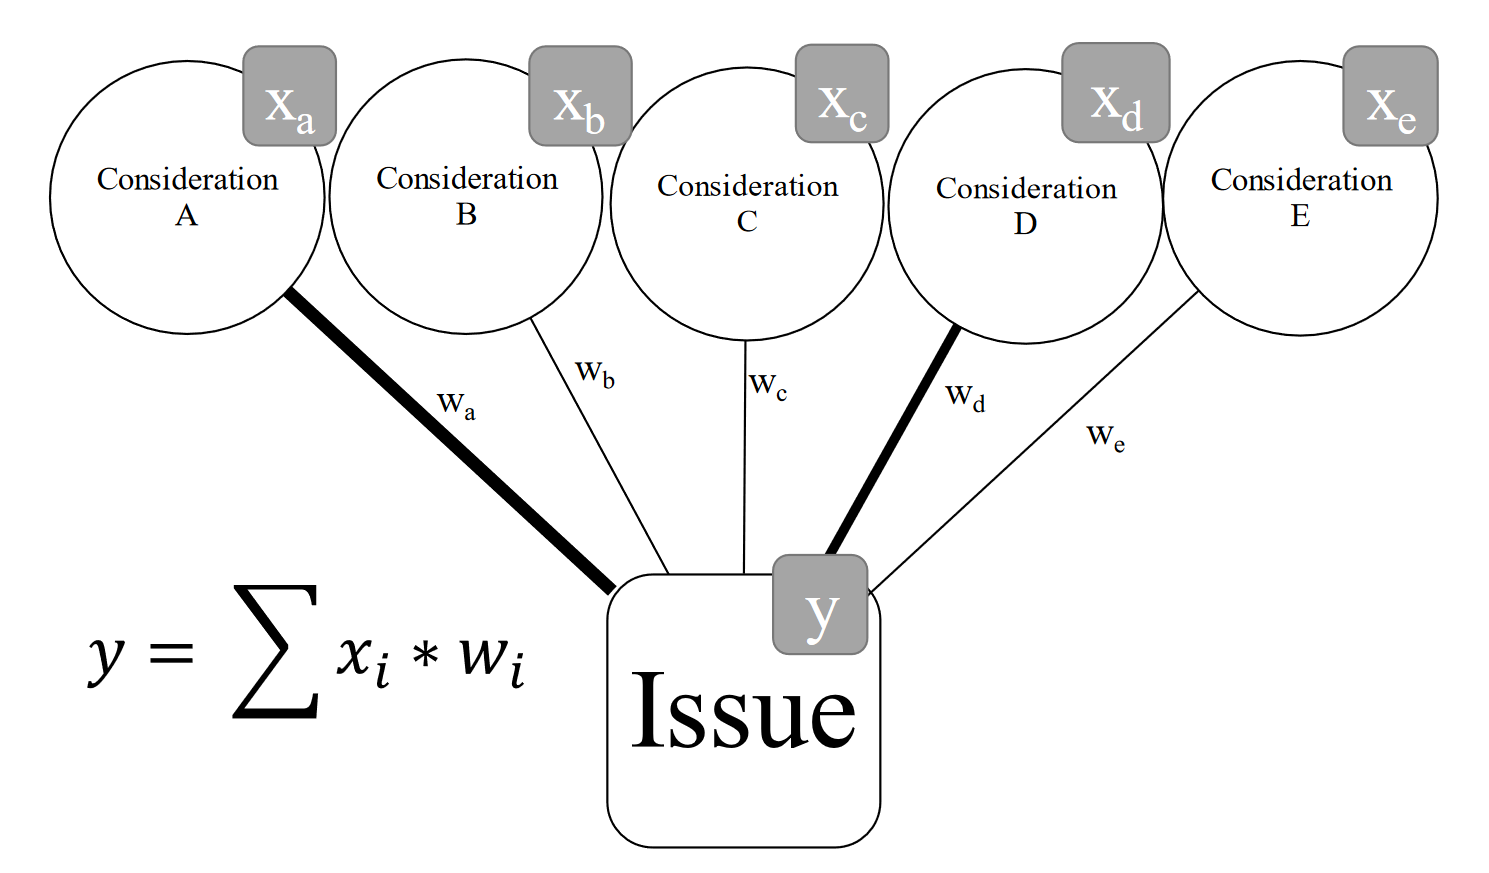
\includegraphics[width=\textwidth]{paper/vis/CognitiveStorage.png}
    \caption{The cognitive evaluation of an issue $y$ is determined by the strength of association $w_i$ with other concepts with existing evaluations $x_i$.}
    \label{fig:cogStor}
\end{figure}

While this broad definition gives a first idea of what framing is about, the concept of emphasis framing has been criticised for being too broad and imprecise to contribute anything meaningful to the field (\cite{Scheufele2012}). To address this shortcoming, I follow the framing literature building on the \textit{value-expectancy model} (\cite{Ajzen2000, Nelson1997}). This model suggests that an attitude on a given issue is a function of two things: considerations and their respective weights. The evaluation of the issue is subdivided into a number of considerations (to which political scientists might refer as "valence issues"), which will be easier to evaluate. For example, to decide whether a lockdown is necessary to battle the spread of Covid-19 in one's country, a person might consider the detrimental short-term effect on businesses and individuals' mental health (negative considerations), as well as the cost of overburdened hospitals and additional deaths (positive considerations, at least with respect to the evaluation of a lockdown). Individuals weigh each of these considerations to form an overall opinion on the subject. 


Figure \ref{fig:cogStor} visualises this logic. A given issue is associated with an attitude $y$. The issue is related to a number of different considerations, each of which carries an associated evaluation $x_i$, e.g. that the prevention of overcrowded hospitals is a good thing. Each of these considerations is more or less associated with the issue. Based on the strength of this association $w_i$, a given consideration's evaluation is more or less reflected in the issue evaluation $y$, which is equal to the weighted sum of considerations. Emphasis framing affects the issue attitude $y$ by changing the weights of different considerations\footnote{Note that this concept of framing is identical to second-level or attribute agenda setting (\cite{Lopezescobar2017, McCombs2000}; see \cite[174]{Mclaren2018} for a discussion of the overlap of these literatures). I will stick to the framing perspective here as the literature is focused on issues rather than candidates' attributes, and the conceptualisation as frame allows to form expectations about citizens' reactions to changing news frames.}.

This operationalisation allows me to generate specific expectations about how frames in the news media affect respondents' issue opinions. When presented with an emphasis frame on a given issue, the respondents' cognitive association of the issue with the emphasised consideration should increase, thus changing the evaluation of the issue by increasing the importance of the consideration. If the consideration is positive (towards the issue), the attitude towards the issue should improve, and the opposite when it is negative. \medskip

\textbf{Emphasis framing hypothesis:} If a newspaper emphasises more positive/negative frames of an issue, the readers' attitude about the issue becomes more positive/negative.




\section{Study design}

\subsection{Public opinion data}

To measure the dependent variable (issue attitudes) and differentiate the treatment groups (newspaper readers), I employ panel data from the German Longitudinal Election Study (\cite{GLES2019LongTermTracking}). Following a period of increased refugee arrivals in Europe in the summer of 2015, the 2017 election was dominated by the migration topic and the related upcoming of the radical-right populist challenger party \textit{AfD}. The major two parties dominating German post-war politics, \textit{SPD} and \textit{CDU/CSU}, had to face severe losses following their 'grand coalition' (\cite{Bieber2021, Wessels2021}). This strong (although still variant, see figure \ref{fig:salience}) salience of the migration issue both in the media as well as in citizens subjective evaluations presents an ideal case to study the effects of shifting media framing on issue attitudes, as continuous coverage on and public debate of the issue are a given.

The panel consists of 15 waves, of which 6 (4) contain variables on newspaper consumption, intended voting decision and immigration (integration) attitudes. In each wave 9,000-15,000 respondents were interviewed, which allows the precise estimation of effects of media consumption. Figure \ref{fig:issues} shows the two main dependent variables for each group of readers. Note that higher values indicate more restrictive attitudes towards immigration/integration (see plot subtitles for more information). As can be seen, readers of the tabloid 'Bild' differ strongly from consumers of other outlets, with far more restrictive attitudes. Both variables seem correlated (as expected), with values moving towards the more liberal pole until autumn, where the trend is reversed.

\begin{figure}[!ht]
    \centering
    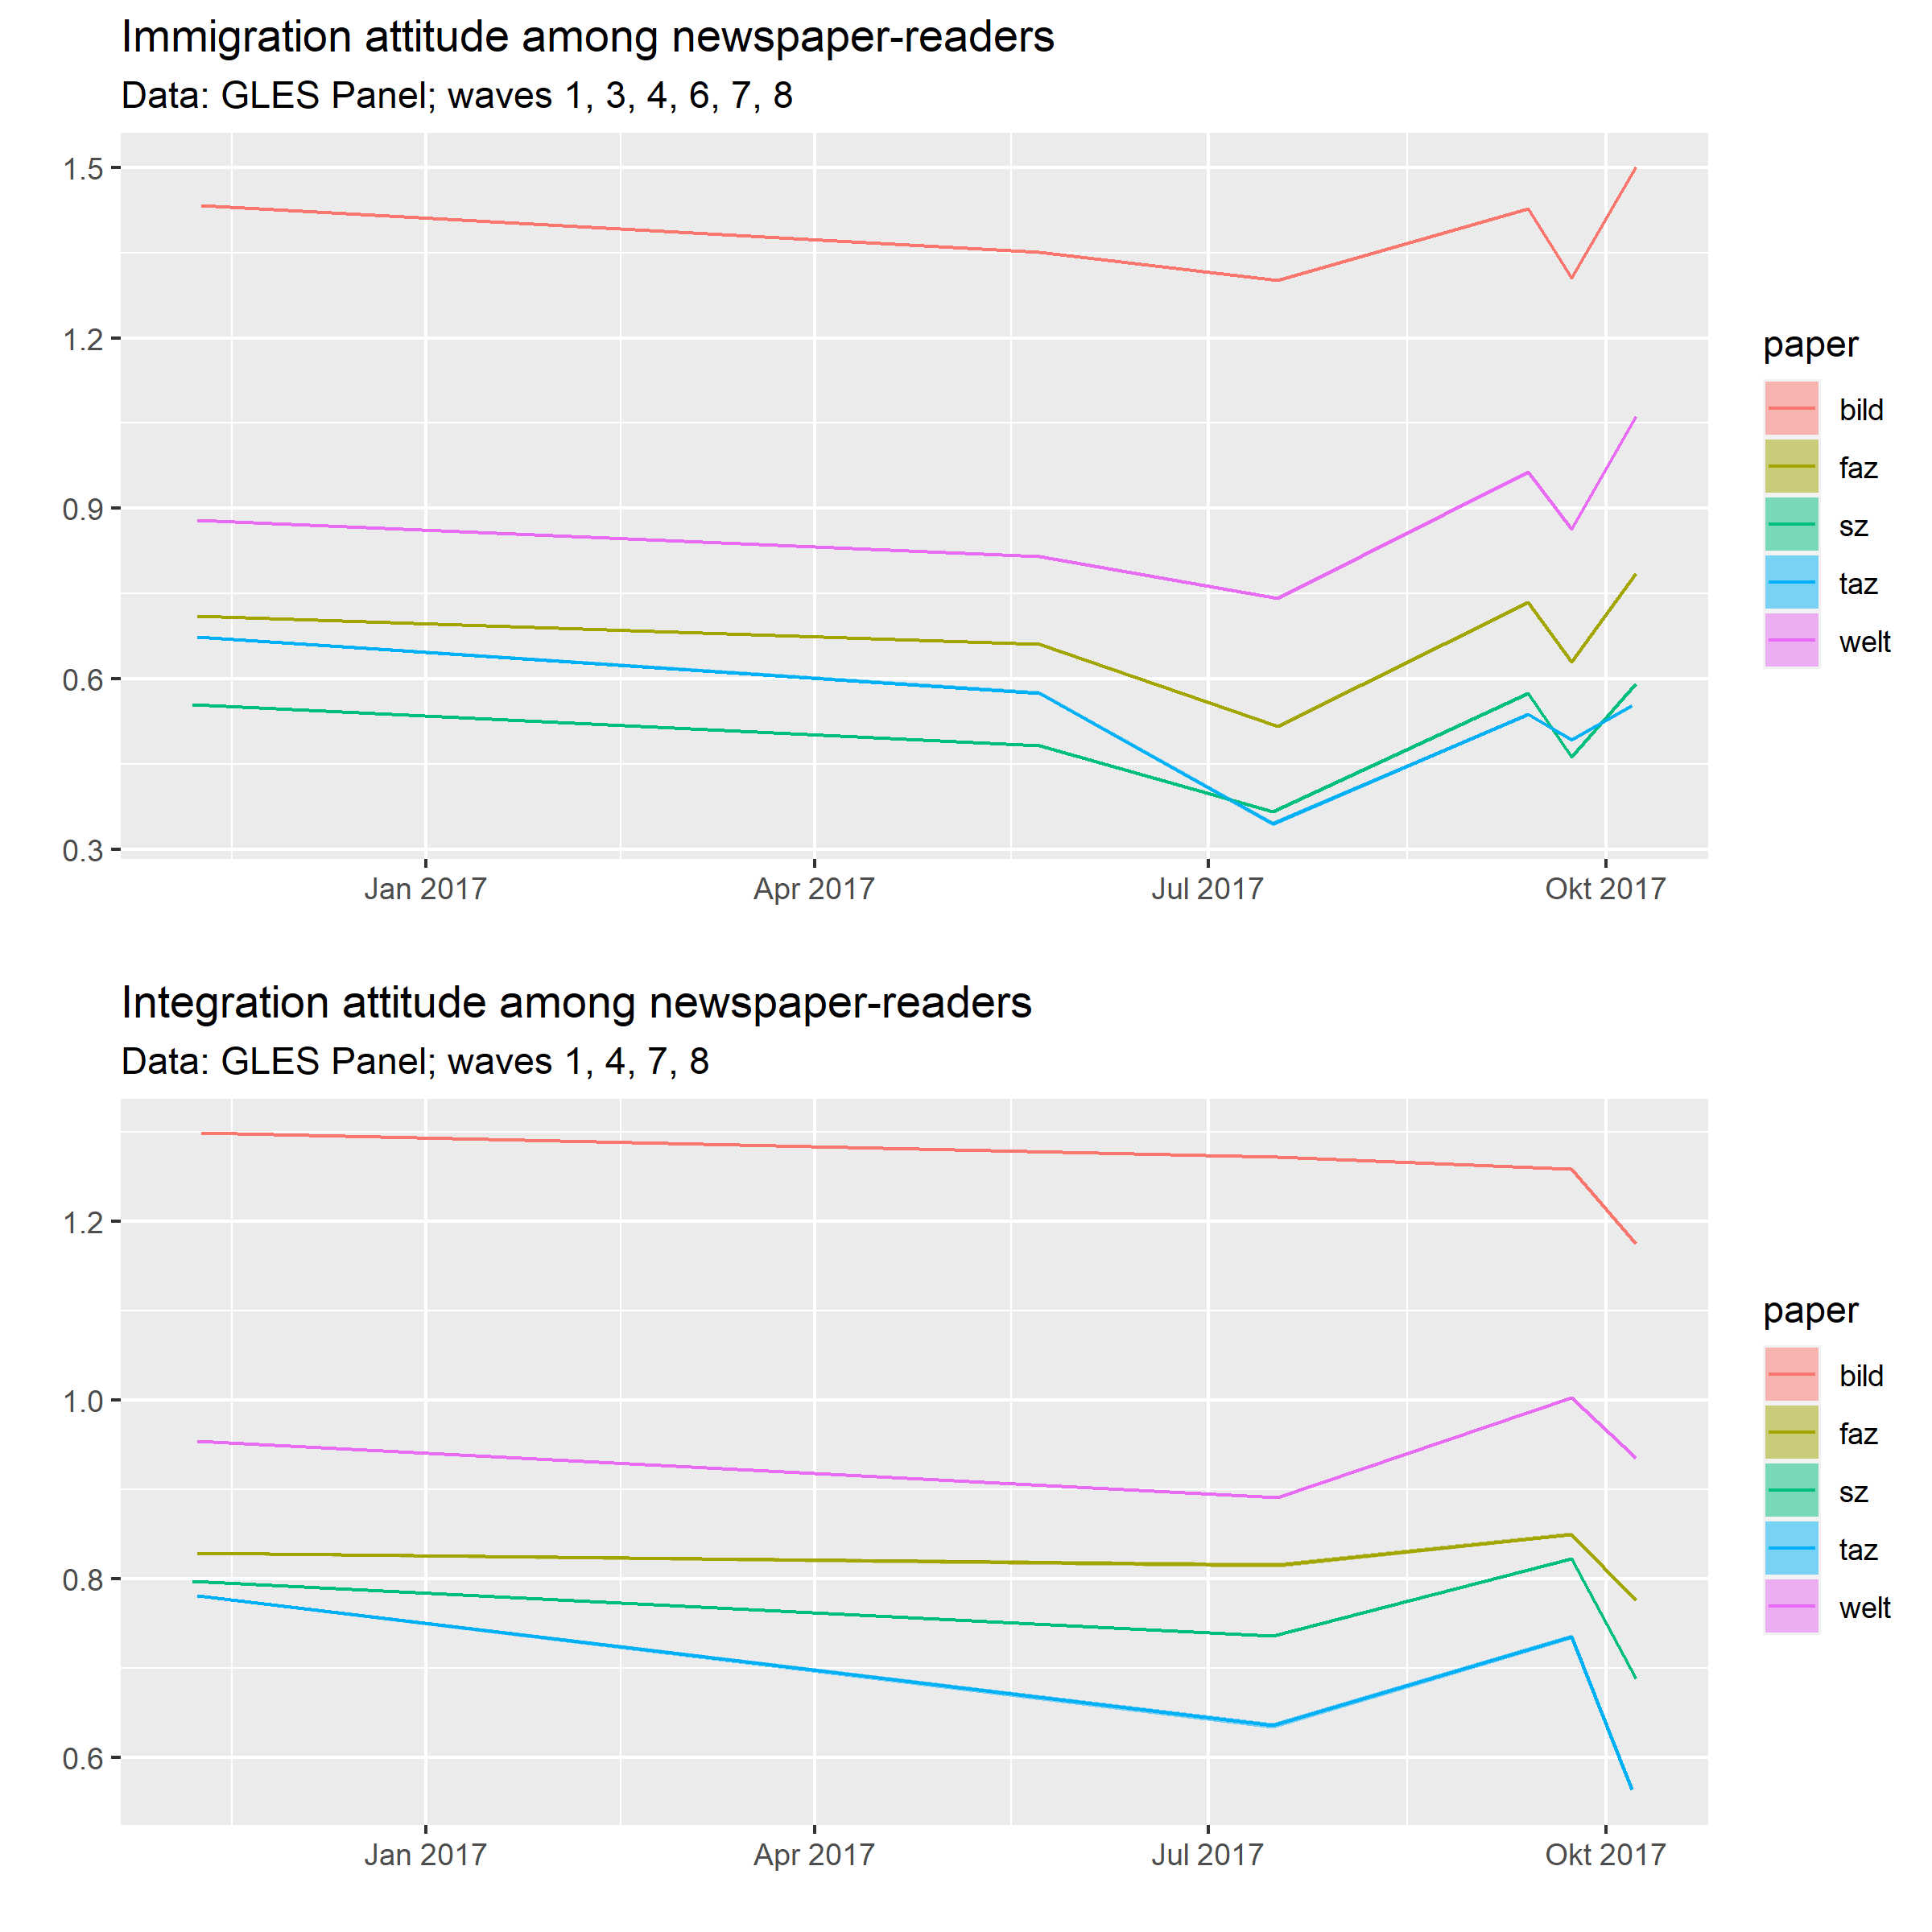
\includegraphics[width=\textwidth]{paper/vis/issues_readers.png}
    \caption{Opinions on migration and integration across time (higher values on immigration indicate more restrictive attitudes, vice versa for integration).}
    \label{fig:issues}
\end{figure}


\subsection{Measuring news framing}

\subsubsection{Measuring news attention to migration}


To measure media attention to immigration, I collected 2.5 million newspaper articles from the most important German broadsheets \textit{Frankfurter Allgemeine Zeitung (FAZ), Spiegel Online (SPON), Süddeutsche Zeitung (SZ), Die Tageszeitung (TAZ), Die Welt} and the major German tabloid \textit{Bild} for the period 2013-2019. Table \ref{tab:paper_sales} shows the number of print copies sold and online page impressions for each newspaper per day. The tabloid \textit{Bild} has by far the largest reach, closely followed by the weekly published \textit{Spiegel}. The daily broadsheets sell less, and interestingly the online presence seems to be dominated by the right, given the weak presence of centre-left \textit{SZ} and \textit{taz}.

\begin{table}[!htbp] \centering 
    \begin{tabular}{@{\extracolsep{5pt}} lcc} 
    \\[-1.8ex]\hline 
    \hline \\[-1.8ex] 
    Paper & Print Sales & Web Impressions \\ 
     & (thousands) & (millions) \\
    \hline \\[-1.8ex] 
    Bild & 1756 & 555 \\ 
    Spiegel & 758 & 388 \\ 
    FAZ & 242 & 123 \\ 
    SZ & 358 & 13 \\ 
    taz & 51 & 7 \\ 
    Welt & 521 & 135 \\ 
    \hline \\[-1.8ex] 
    \end{tabular} 
  \caption{Average daily sales and online impressions of different newspapers in 2017. Source: \cite{IVW}. Table generated with stargazer (\cite{stargazer}).} 
  \label{tab:paper_sales} 
\end{table}

To identify whether an article is about migration, I train a BERT deep-learning classifier. As migration content is rare, and my training data needs to be somewhat balanced, I first construct a dictionary of terms related to migration. I use dictionary extension based on German GloVe word-embeddings\footnote{Downloadable from \url{https://deepset.ai/german-word-embeddings}.} to construct a comprehensive dictionary, and apply it to the articles. Based on the relative share of migration words in an article, I draw a stratified sample of 300 articles (100 from the third with fewest migration terms, 100 from the third with most migration terms and 100 from the third in between) for each newspaper for a total of 1,800 papers. Then, a student assistant\footnote{Thank you, Robin. I know it was painful.} hand-coded these articles, assessing whether their main topic is related to migration. 

Using this sample, a BERT deep-learning classifier\footnote{\url{https://huggingface.co/bert-base-german-cased}} is fine-tuned on a subset of 1,400 annotated articles. After fine-tuning, the model correctly classifies 95.5\% of the test set (F1: 0.94, recall: 0.93, precision: 0.95). This classifier is then used to annotate all 2.5 million newspaper articles. For the time frame from 2013 to 2019, around 90,000 (3.6\%) are identified to treat the issue of migration.

\begin{figure}[!ht]
    \centering
    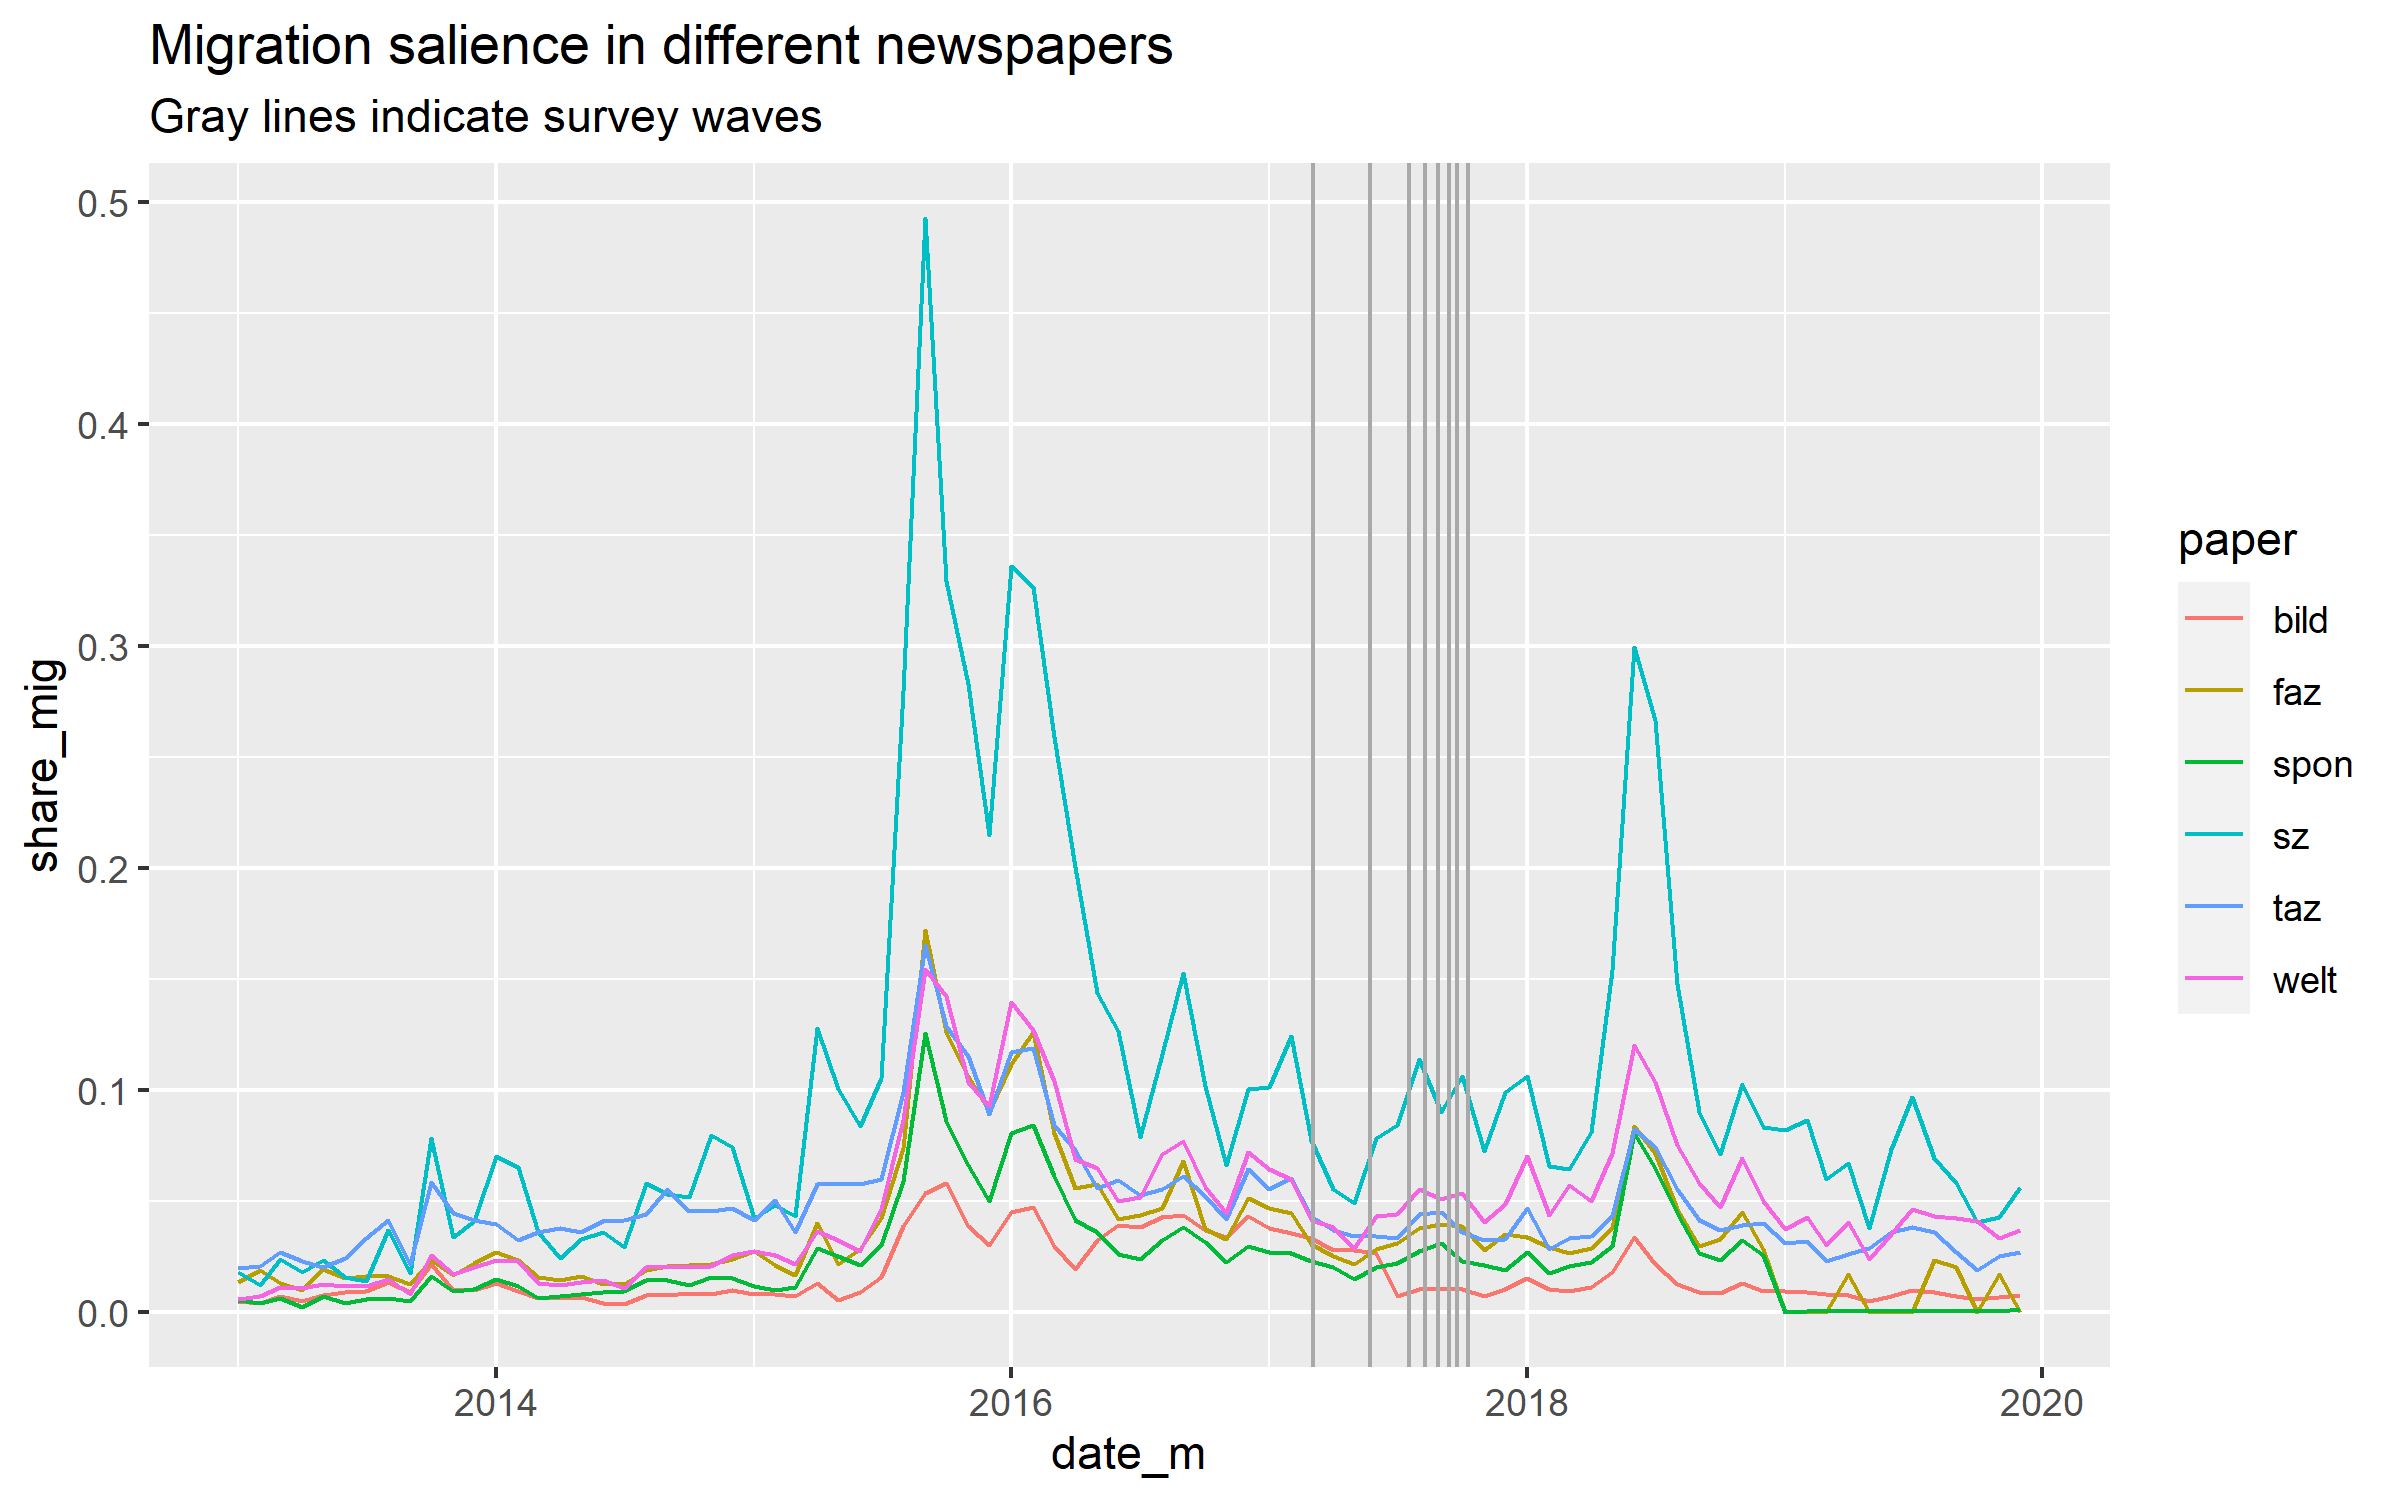
\includegraphics[width=\textwidth]{paper/vis/salience_papers.png}
    \caption{Share of migration articles out of all articles across time for different newspapers.}
    \label{fig:salience}
\end{figure}

Figure \ref{fig:salience} shows the share of migration articles in each newspaper. Clear peaks in attention are visible surrounding the refugee movements of summer 2015, following the new years eve in Cologne 2016, and the conflict over asylum policy between CDU and CSU in 2018. Newspapers seem to be event-driven and follow largely parallel trends, albeit at different levels, with the  centre-left \textit{SZ} discussing migration most and the tabloid \textit{Bild} least. Attention decreases in mid-2016, but remains high compared to pre-2015 levels. Surrounding the fielding period of the survey waves (gray vertical lines), most newspapers show similar levels of attention to the issue between 2.5\% and 6\% of all articles, with the exception of \textit{SZ}, which moves between 5\% and 12.5\%.



\subsubsection{Measuring news frames}\label{sec:frame_selection}

To measure news frames, I estimate a structural topic model with 60 topics for the nearly 90,000 migration articles in the full period (2016-2019)\footnote{The topics' prevalence along with the most important words can be assessed in appendix \ref{app:stm}.}. The number of topics was chosen to strike a balance between the computational and human resources necessary to estimate and annotate the topics and finding appropriate topics for the large corpus of nearly 90,000 migration articles. Topic prevalence is estimated as a function of the release date of the article, as well as the newspaper it has been published in. The 60 topics' most predictive words and ten most representative articles were assessed to identify and label the content of each topic, and the most frequent and relevant topics that allow to form clear hypotheses regarding their effect on immigration attitudes are selected. 

With this procedure, the following seven 'large' migration frames were selected (number of topic added corresponds to the graph in appendix \ref{app:stm}):

\begin{enumerate}
    \item Capital crime (sexual assault/rape/murder) committed by refugees (topic 48), 
    \item illegal entry and petty crime (topic 25),
    \item refugee numbers (topic 32),
    \item labour market needs for and job market integration of refugees (topic 11),
    \item deportations (topic 44),
    \item internment camps (e.g. Moria; topic 27),
    \item drownings in the Mediterranean (topic 49).
\end{enumerate}

I expect the capital crime, illegal entry/petty crime, and the refugee numbers frames to have negative effects on attitudes towards migrants (as connected to negative considerations regarding immigration), while deportations, internment camps, and drownings in the Mediterranean sea should have positive effects, framing immigration as a humanitarian issue. The labour market frame should show mixed results, given that labour market integration might be perceived as threatening or addressing needs in the German economy. Figure \ref{fig:frames} shows the prevalence of these frames across time for each newspaper. It can be seen that substantial variation exists in the relative emphasis of migration frames both within and across newspapers. Interestingly, some issues seem to vary according to newspaper slant. For example, more right-leaning outlets \textit{Bild, FAZ}, and \textit{Welt} seem to largely emphasise crime and deportations, compared to their centrist and left-wing competitors. This lends some first credibility to the expected effects for these frames, although the differences are not clearly visible for the other frames.

\begin{figure}[!ht]
    \centering
    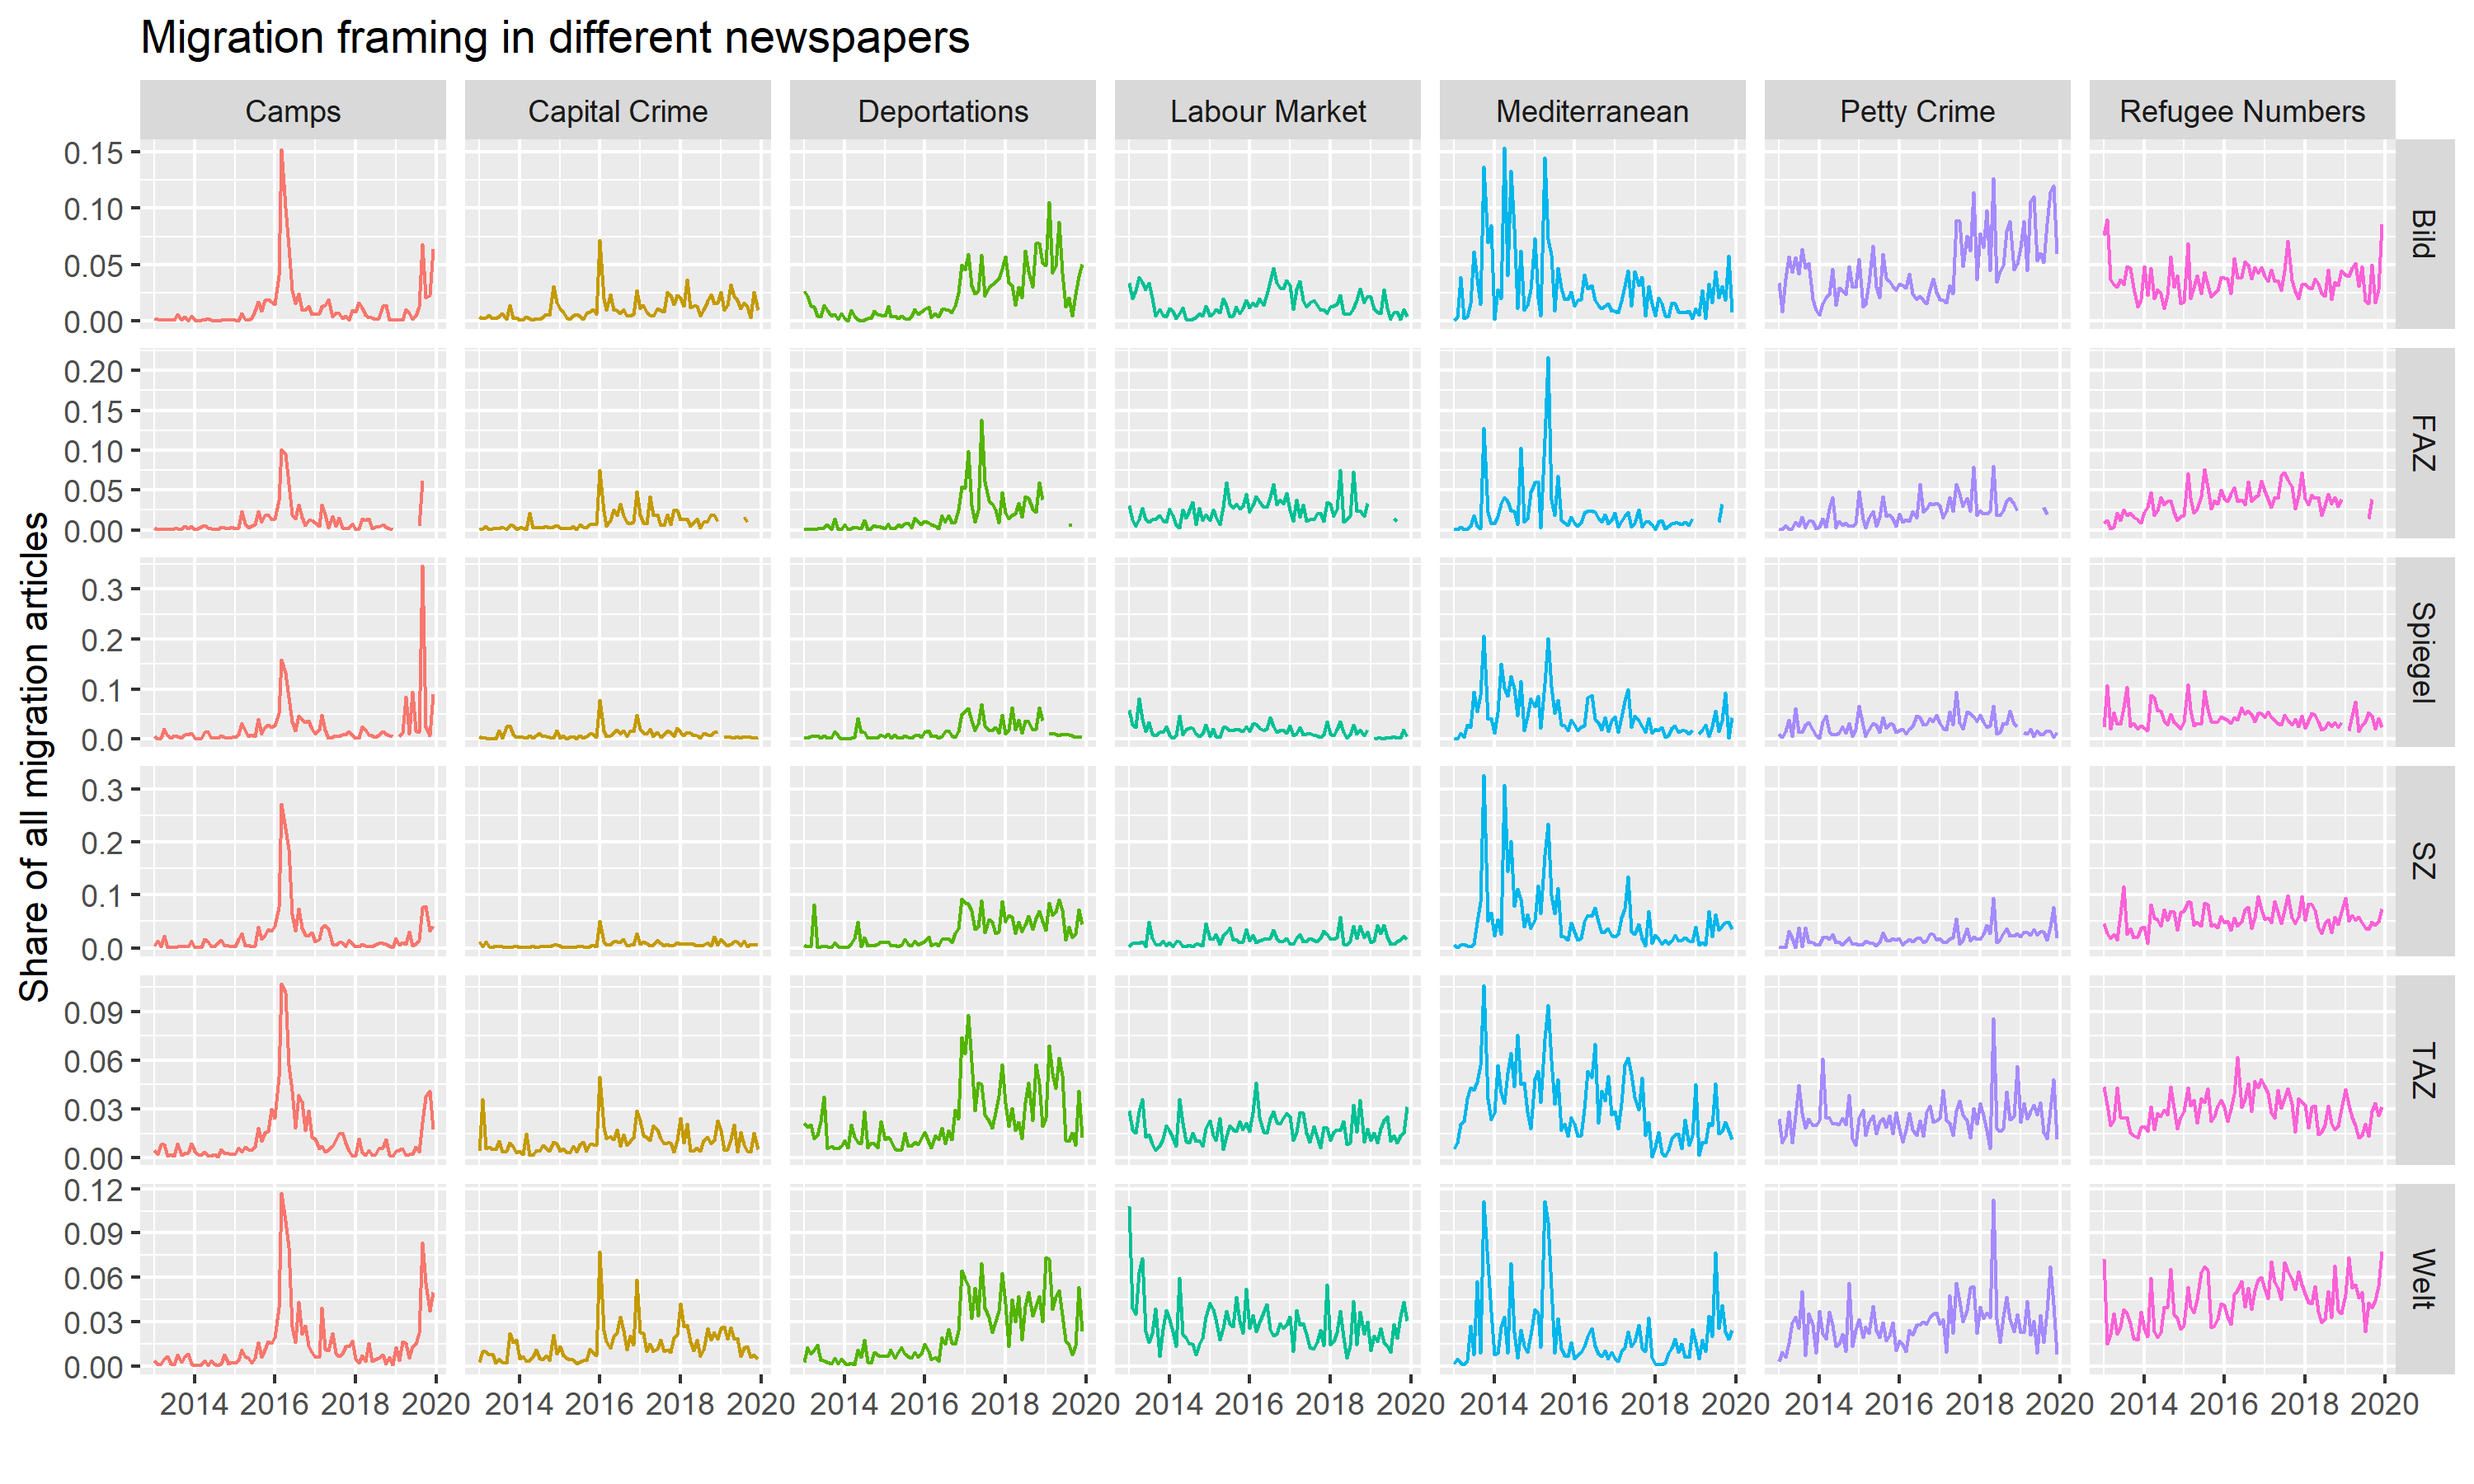
\includegraphics[width=\textwidth]{paper/vis/frames_papers.png}
    \caption{Prevalence of different migration frames across newspapers and time.}
    \label{fig:frames}
\end{figure}

\subsection{Local data on news exposure and voting behaviour}

I am in the process of collecting data on the distribution of different newspapers in German electoral districts, as well as data on voting behaviour within these districts. This allows to assess whether higher readership of \textit{Bild} (and thus more exposure to its migration framing) results in changes in voting behavior following the change in migration framing after the editor-in-chiefs departure (see below) and the subsequent change in migration framing. 

\section{Case description and treatment}

During the summer of 2015, the German tabloid Bild responded to the emerging migration issue unexpectedly progressive, calling for support for the newly arriving immigrants and attacking those promoting hate against refugees online (Bild stellt Hetzer an den Pranger 2015; Alvarez 2015), before starting the campaign ’We help - \#refugeeswelcome’ (Grosse Bild-Aktion: Wir helfen - \#refugeeswelcome n.d.). With this move, the paper heavily diverged from its right-wing tradition. The major change in tone was largely ascribed to then editor-in-chief Kai Diekmann, who had also invited a refugee family to live in his house (Reichart 2015). Diekmann left the company in January 2017. Then sole Bild editor-in-chief Julian Reichelt increasingly painted a picture of refugees as criminals and terrorists on the tabloid's front page (Niggemeyer 2018; Zudeick 2018). I aim to exploit this communicative shift in the tabloid’s migration framing to assess the effects of media framing on readers’ issue definitions, attitudes, and voting behaviour. As figure \ref{fig:frames_diekmann} shows, the migration framing presented in Bild changed following Diekmann's departure. Specifically, immigration was increasingly framed in terms of crime, while other newspapers maintained their levels of attention (see also figure \ref{app:diekmann_all_frames} in the appendix).

\begin{figure}
    \centering
    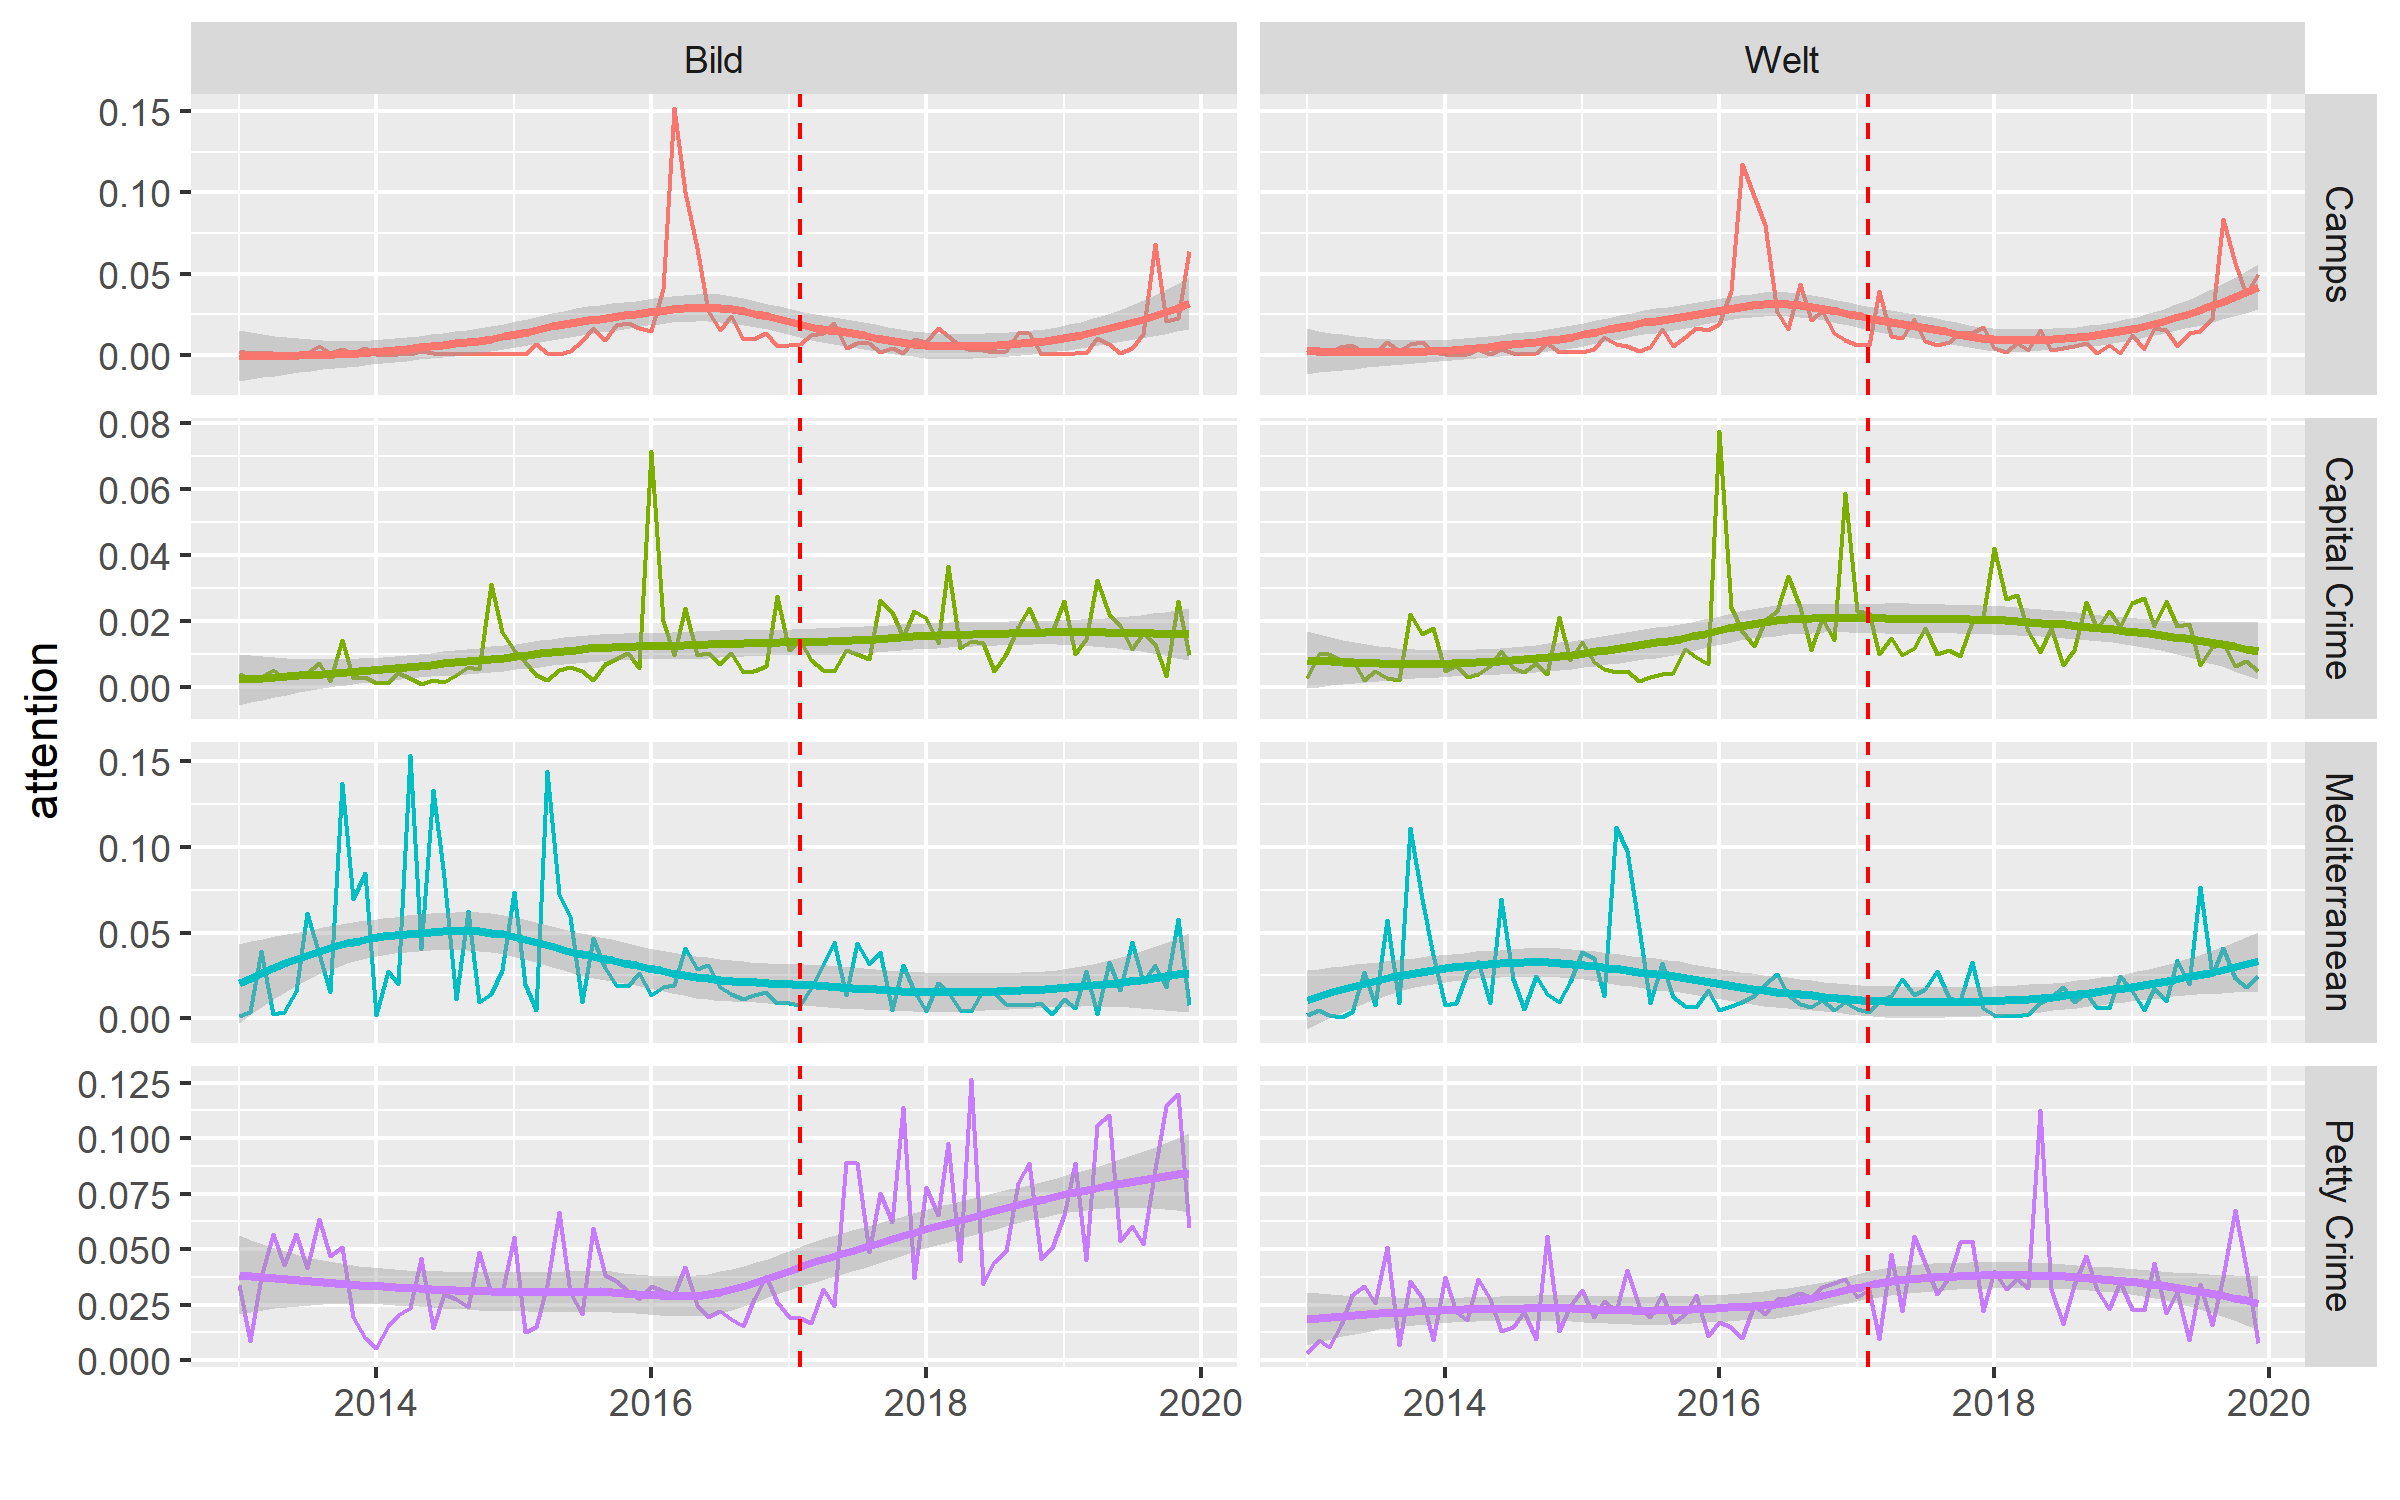
\includegraphics[width=\textwidth]{paper/frames_bild_diekmann_pres.png}
    \caption{Monthly attention to different immigration frames following departure of Diekmann from Bild, for Bild and Welt. While attention to other frames follows the Welt's coverage of immigration (or any other newspaper, see appendix \ref{app:diekmann_all_frames}), an increase in Bild attention to general crime news when reporting about immigration is visible following the departure of Diekmann.}
    \label{fig:frames_diekmann}
\end{figure}

Both studies in this paper build on this shift in attention. Study 1 will present estimates from two models assessing whether changing attention to any frame will affect issue attitudes or voting behaviour, using media and opinion data on the migration issue from the German national election in 2017. This is followed by a Difference-in-Difference estimate based on the change in attention to the crime frame presented above. Study 2 will turn to behavioral data and assess whether voting behaviour in voting districts with more circulation of \textit{Bild} have experienced changes in voting behaviour.



\subsection{Estimation}

\subsubsection{Differences in opinion formation across readers}\label{sec:did_readers}

To assess whether opinion shifts might be influenced by news consumption, I isolate the opinion shift by readers of one newspaper relative to all other newspaper readers. To do this, I estimate difference-in-differences (DiDs) for all available combinations of issues, news outlets, and survey waves. The binary variable indicating readership controls for differences in levels between different news consumers, while the binary variable indicating the survey wave controls for general attitudinal shifts across time. The main term of interest is then the interaction of the binary indicator of readership of a certain outlet with the binary indicator for the current wave. This captures the change of the specified group (e.g. \textit{Bild}-readers), beyond time-constant differences between the newspapers and general trends from one survey wave to another. Hence I measure the shift in opinions of the readership of a certain outlet, controlling for the changes taking place among consumers of other news. The formula is given below:

$$ y = \beta_1 * W + \beta_2 * R + \beta_3 * W * R, $$

where $y$ is the dependent (migration opinion), $W$ indicates whether the interview took place ($W = 1$) in a given survey wave or in the preceding one ($W = 0$), and $R$ indicates whether the respondent is a reader of the newspaper of interest.


\subsubsection{Estimation of framing effect}\label{sec:models}

I estimate the same DiDs to measure shifts in migration framing in a given newspaper, controlling for shifts in all other newspapers. To do that, I first sum the attention given to a certain frame in a given newspaper in the past day, week, month, or half year, up to the last survey wave. This allows me to assess whether choosing different lags affects my estimates. Then, I estimate the DiD, indicating how much a newspaper changed its attention to a given migration frame, relative to all others. The DiDs estimating the opinion shifts described in \ref{sec:did_readers} are then matched and regressed on the shifts in migration framing. If increasing attention to a certain frame causes a shift in migration attitudes, these two measures should be highly correlated.

Second, I fit two-way fixed-effect models with individual news framing estimates for each survey interview. Since waves are sometimes fielded for several weeks, it might be a strong assumption to treat all interview dates within a given survey wave as identical. I measure exposure to each frame by summing up the frame attention of the past week (relative to the individual interview) in each newspaper the respondent claimed to have read in the past week and dividing it by the total number of newspapers read. This way, I estimate frame exposure for each individual respondent's interview date and news diet, which allows to estimate the correlation of changes in immigration opinion with the migration framing in recently consumed outlets.

While the DiD's are better identified, controlling for shifts in other newspapers and reader groups, they suffer from the fact that surveys are conducted for several days, often up to two weeks, which makes the precise matching of newspaper content impossible. The fixed-effect models control for wave effects and (time-constant) individual characteristics, therefor restricting the explainable variance to everything beyond general trends and individual characteristics, but might include more noise. Another difference is that the DiD-models correlate changes, while the fixed-effect models regress opinion levels on frame attention levels.

\subsubsection{Local changes in voting behaviour}



\section{Results}

\subsection{Study 1}

\subsubsection{Correlation of opinion changes among readers with changing frame attention in consumed newspapers}

As figure \ref{fig:issues} shows, and as discussed in appendix \ref{sec:did_ass} and \ref{sec:did_sig}, the dependent variables show highly parallel trends but also display considerable variation beyond statistical noise\footnote{Recent, additional analyses have shown that the opinion shifts vary beyond statistical noise only when considering the broadly defined treatment (all readers of a newspaper). If however consulting only changes among those consuming a single newspaper, significance levels of these shifts approach what would be expected through random sampling error (see figure \ref{fig:did_by_treat}). At this point, it is unclear whether this is an outcome of severely decreased sample size or lack of opinion change among exclusive readers.}
. Can these opinion shifts be explained by shifts in news content? Figure \ref{fig:did_corr} shows the core analysis to estimate the effect of migration framing on reader opinion. The displayed estimates are obtained by regressing the DiD-estimates for issue attitudes on the DiD-estimates for media attention, as described in section \ref{sec:models}. If opinion shifts among newspapers' readers - relative to other readers - can be explained by shifts in newspapers' issue framing, these two variables should be highly correlated.

\begin{figure}
    \centering
    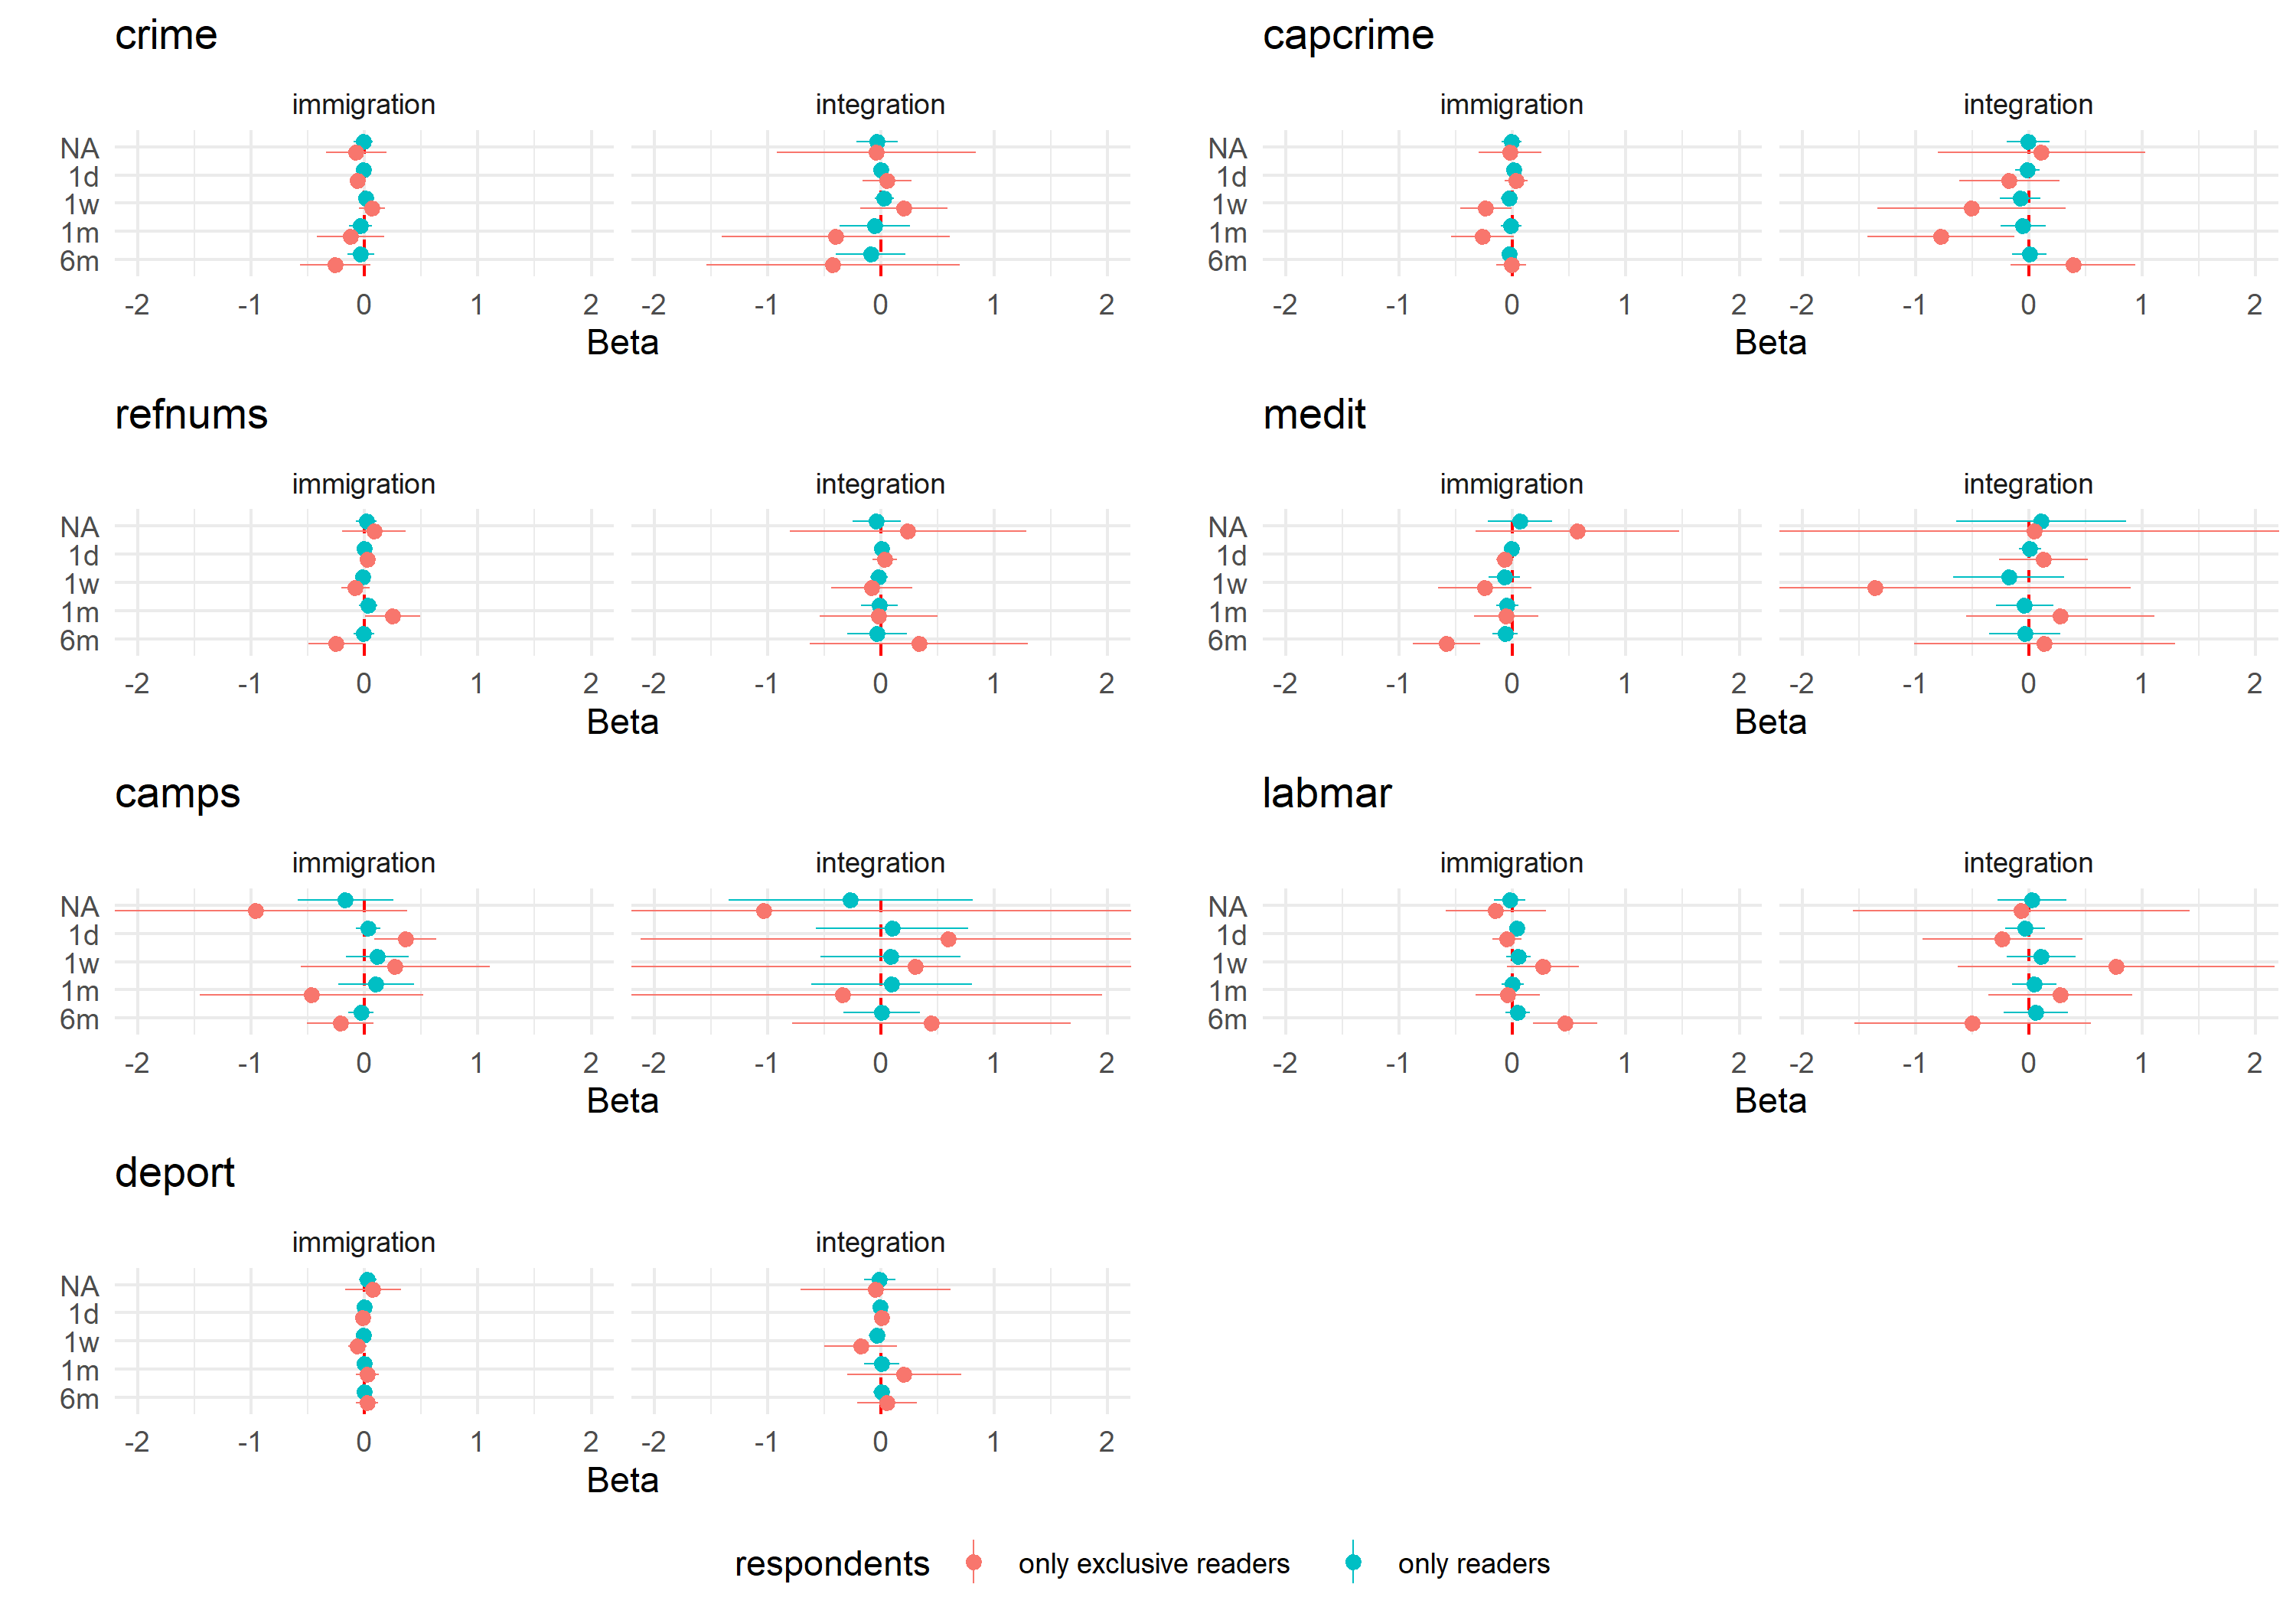
\includegraphics[width=\textwidth]{paper/vis/effectplot_frames_did.png}
    \caption{Regression coefficients from DiD-models with different specifications.}
    \label{fig:did_corr}
\end{figure}

This is however not the case. Each panel in figure \ref{fig:did_corr} shows the effect of one frame on an attitude variable and the intention to vote for the radical right \textit{AfD} (controlling for all other frames mentioned in section \ref{sec:frame_selection}), across different lags and treatment definitions. Each dot in this graph represents the coefficient of a model explaining standardised\footnote{Meaning that independent and dependent variables were mean-corrected and re-scaled to standard deviations before regression. A coefficient of one means that a one-standard-deviation shift in the independent variable corresponds to a one-standard deviation shift in the dependent variable.} aggregate opinion shifts with standardised shifts in media attention to specific frames.  For example, in the upper left panel 'crime', we can see three different panes ('afd-support', 'immigration' and 'integration') for each dependent variable. The vertical rows distinguish four different lags indicating the frame prevalence of the past day, week, month, half year, or the entire period up to the last survey date. Additionally, the color of the points indicates whether the model was estimated only for readers of a single newspaper (lower N, but no treatment diffusion) or all readers of a newspaper (who might read another newspaper, say SZ readers who also read FAZ). 

Only very few estimates are significant and no trends emerge across specifications for any variable. All estimates are clustering around zero, indicating no effect. Estimates of all relationships indicate both positive and negative relationships across specifications. While the 'exclusive reader' estimates show more variation, they also indicate far broader confidence intervals. There is no considerable difference across lags, and the variables only differ by the broader confidence intervals of the integration variable, owing to the fewer waves including this question. Generally, this analysis indicates no effect of media framing of migration on migration attitudes or voting behaviour.

\subsubsection{Fixed-effect model}

To corroborate these results, I estimate another model directly regressing individual migration opinions on individual estimates of consumed migration frames with fixed effects for survey wave and respondent (see section \ref{sec:models}). The results for migration and integration attitudes can be seen in figure \ref{fig:model_fe}.

Again, most estimates are not significant, differ in direction across specifications, and cluster around zero. While some estimates are unidirectional (crime and labour market on the immigration issue; crime, capital crime, labour market and camps on \textit{AfD}-support), they show tiny effects (a standard deviation increase in attention to the labour market makes immigration attitudes between 0.005 and 0.015 standard deviations more conservative) and are usually not significant. Most importantly, both models do not correspond to expectations. This is probably most visible for the capital and sex crime frame ('capcrime'), which should show strongly positive effects (leading to more restrictive attitudes), but also for the illegal immigration and petty crime frame ('crime'), which consistently shows insignificant negative (i.e. liberalising) effects, contradicting the more sensible increase in \textit{AfD}-support when exposed to this frame.

\begin{figure}
    \centering
    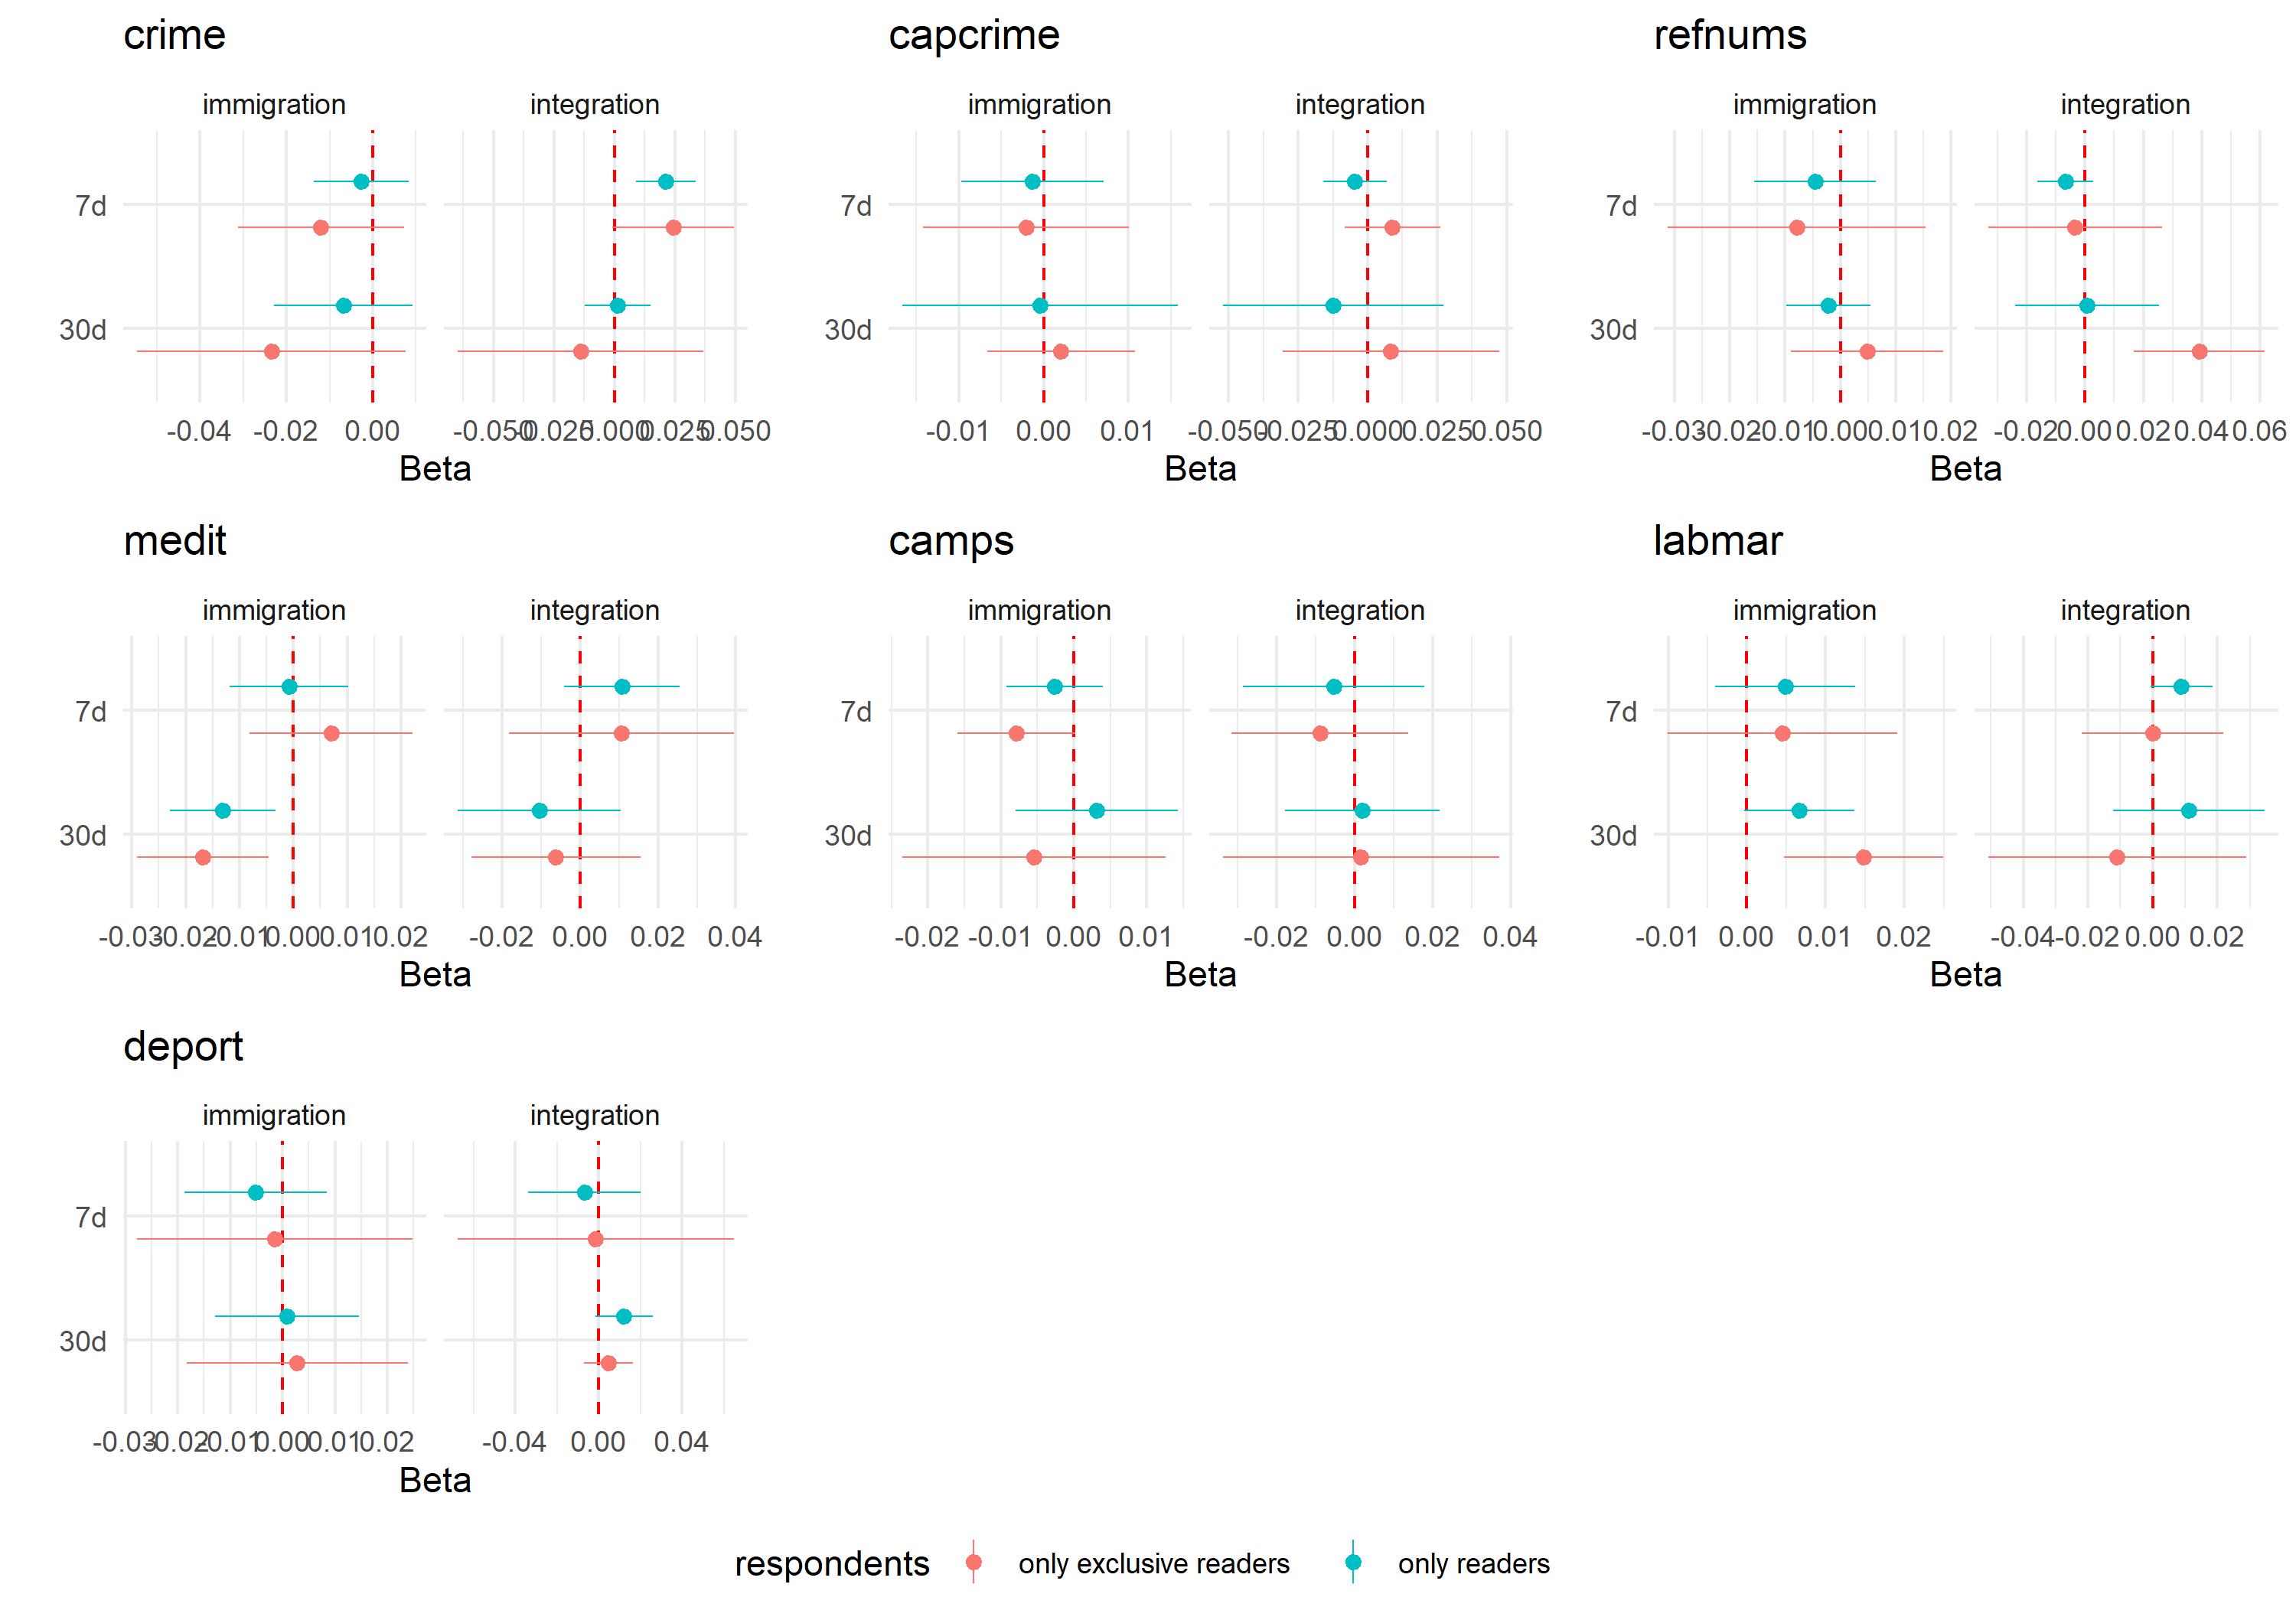
\includegraphics[width=\textwidth]{paper/vis/effectplot_frames_fe_abs.png}
    \caption{Regression coefficients from fixed-effects models with different specifications.}
    \label{fig:model_fe}
\end{figure}

\subsubsection{Difference-in-Difference estimate}

I initially hoped to match former and current readers of Bild or at least readers of Bild and other outlets to assess whether this shift in framing of a single newspaper affected attitudes and voting behaviour. Regrettably, only one survey wave preceded the departure of Diekmann, precluding a test of the parallel trends assumption. However, even under this strong assumption the estimate might be of interest. At this point, however, I can not present such an estimate yet.

\subsection{Study 2}

Results for local differences in electoral behaviour will be added once the data on local news circulation is available.

\section{Discussion}

This paper assesses the responsiveness of newspaper consumers' migration attitudes to the migration framing of their respective newspaper. Aggregate difference-in-differences models and individual estimates show that consumers' opinions on immigration and integration were not reacting to changes in the newspaper framing of the respective issue. These findings add to an increasing body of evidence showing the absence of short-term media effects in contemporary media environments (\cite{Arceneaux2013, Durante2012, Gentzkow2010, Guess2021, Lau2021}). 

Future research will have to establish whether media consumers react to attitude-discrepant information by changing the outlet instead. Several studies found that, instead of reacting with opinion shifts, readers might change their political preferences or mobilise to vote (\cite{Stetka2020}). Similarly, several studies indicate that changes in a media outlet's slant will result in a change in the composition of the consumers (ie those with conflicting attitudes stop reading the newspaper) rather than a change in a fixed readership's attitudes (\cite{Arceneaux2013, Durante2012, Spirig2020}). Whether similar effects can be observed when explicitly measuring newspaper framing are likely next steps for analysis.

If short term changes in framing have no effect on attitudes in the short run, decreases in readership might lead to long-term changes in political opinions due to generational replacement into a changing media environment. This could also make findings from some studies in the field convincingly showing effects (\cite{Foos2020}) consistent with this study and other literature showing weak or absent effects.

Another way forward might be to test theories of \textit{issue evolution} (\cite{Carmines1986}). For example, if a process of 'issue-sorting' took place on the migration issue in 2015, when the topic became very salient, citizens might have chosen a side and stuck to their opinion afterward. Future studies could hence try to identify such windows of opportunity where media effects might still be relevant.

\printbibliography


\section{Appendix}

\subsection{Change in Bild framing of migration issue}

\begin{figure}[!ht]
    \centering
    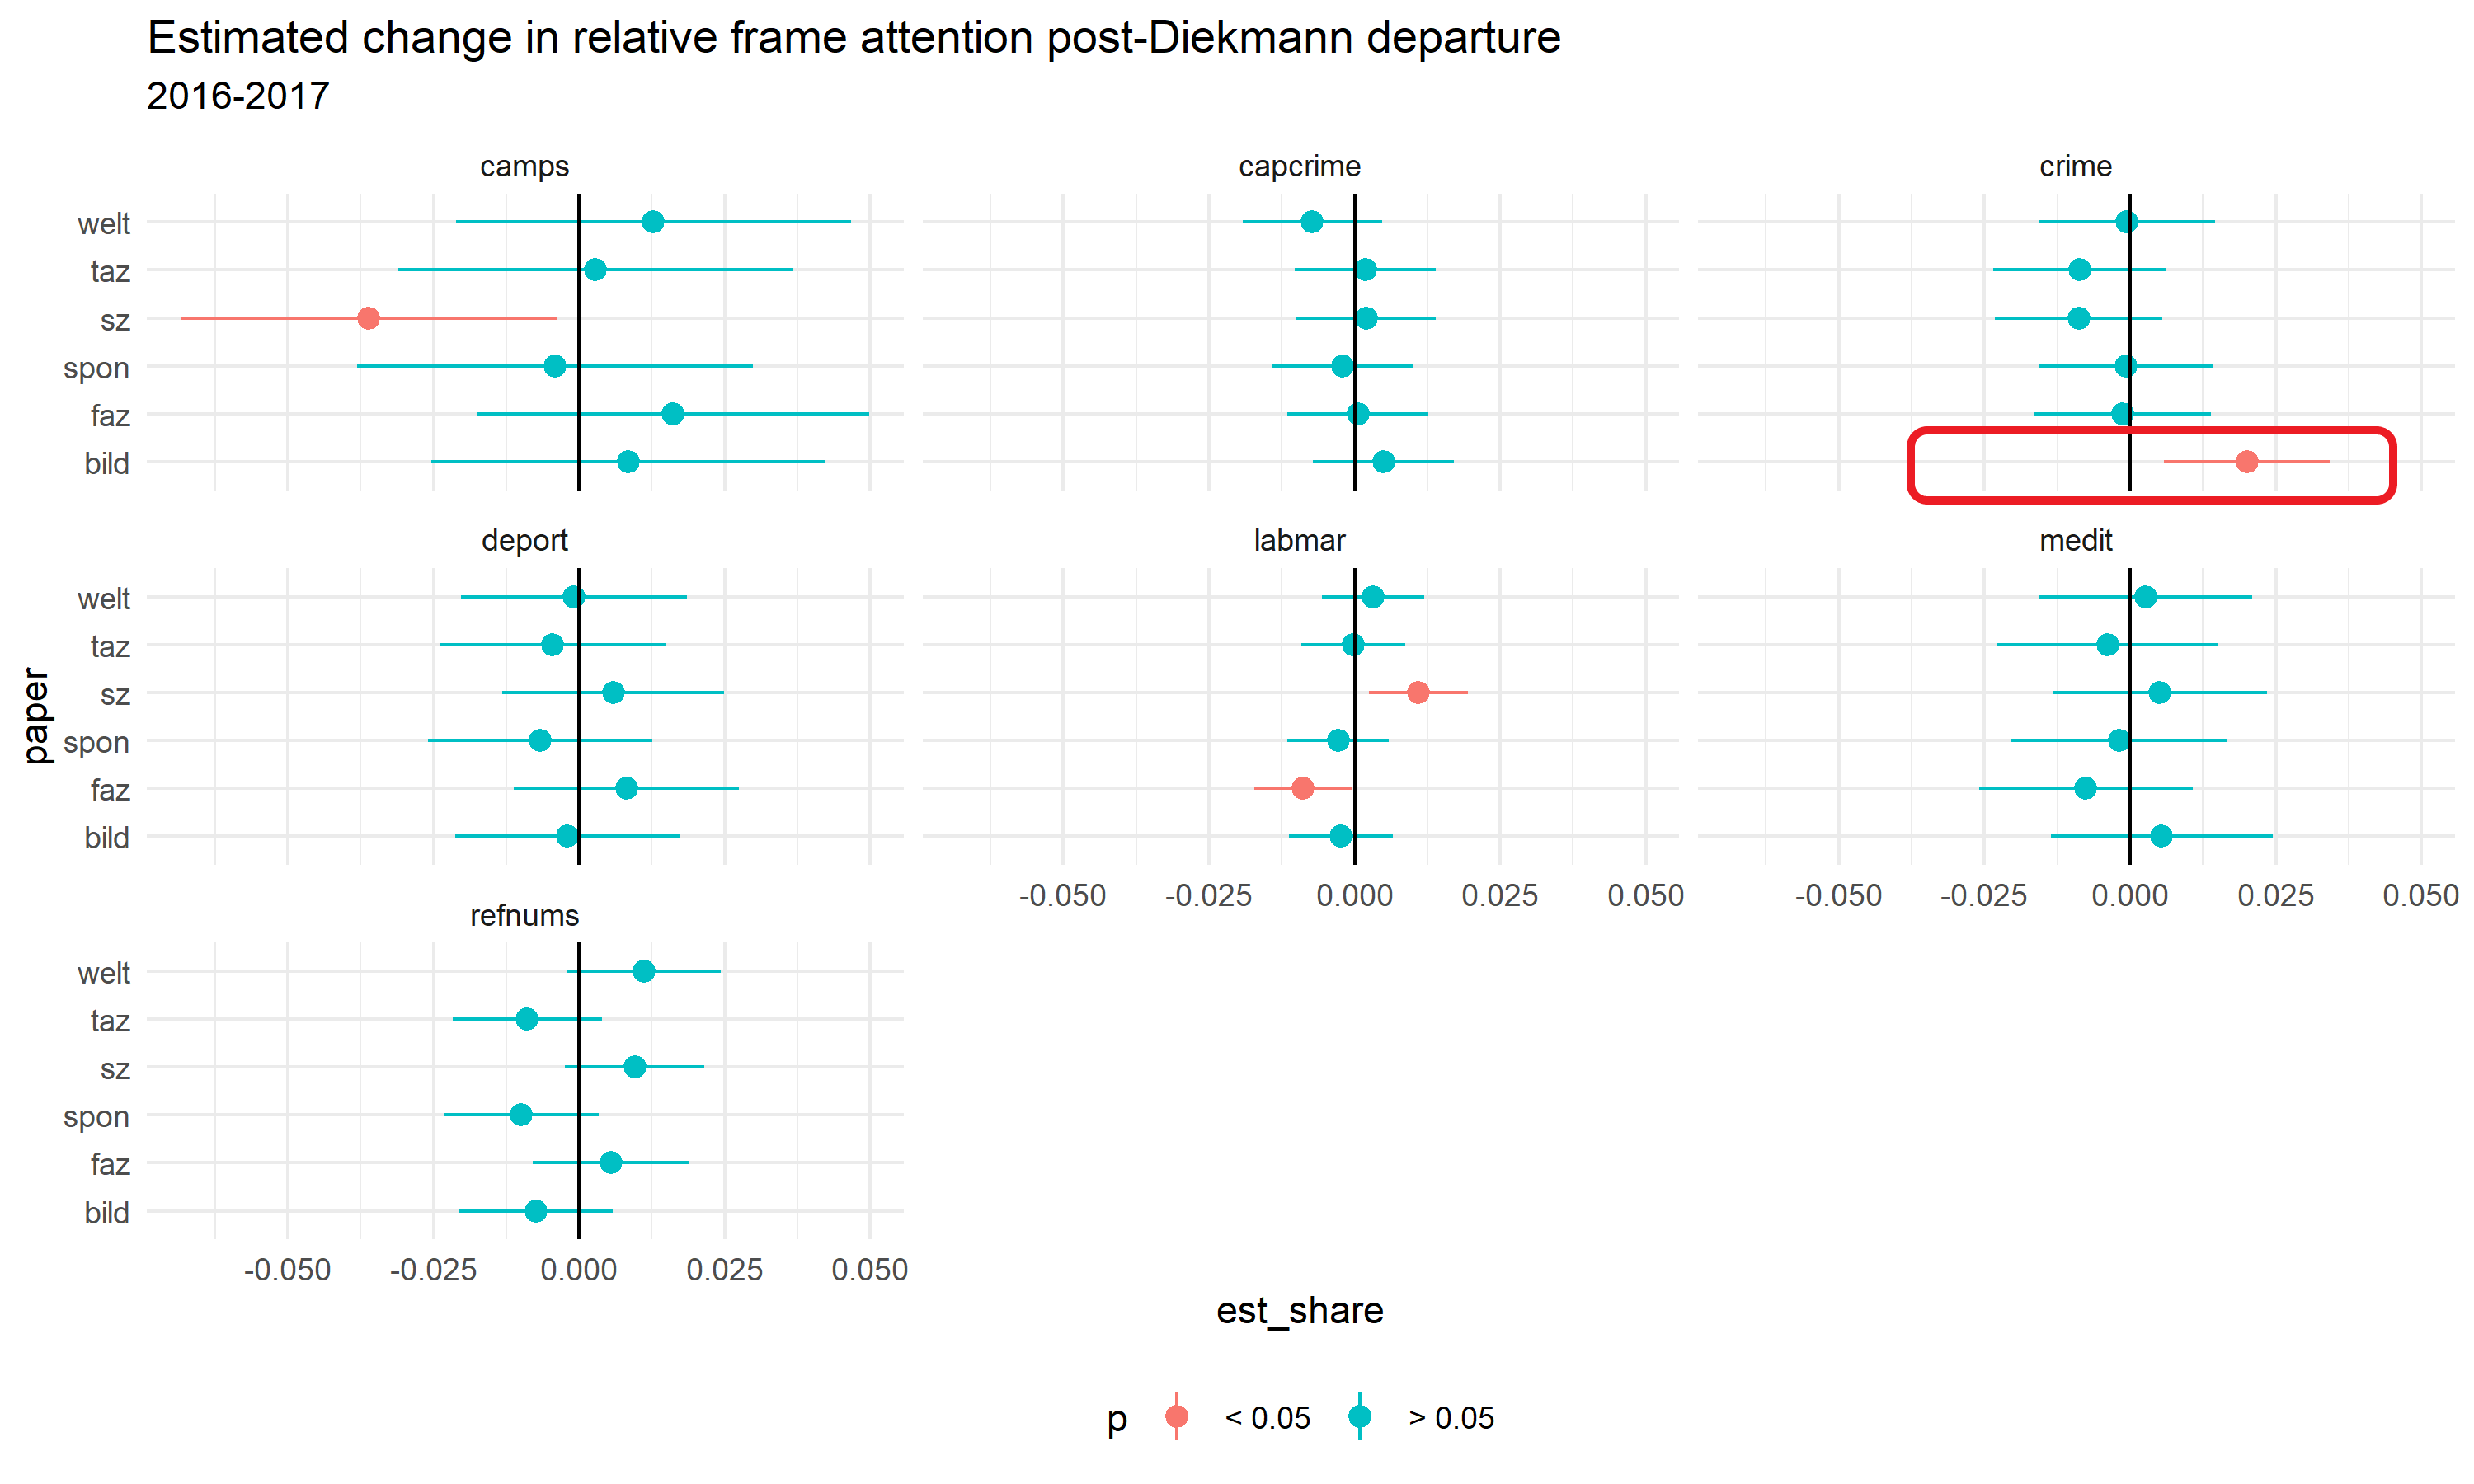
\includegraphics[width=\textwidth]{paper/vis/did_papers_frames_1617_scatter.png}
    \label{app:diekmann_all_frames}
\end{figure}

\begin{figure}[!ht]
    \centering
    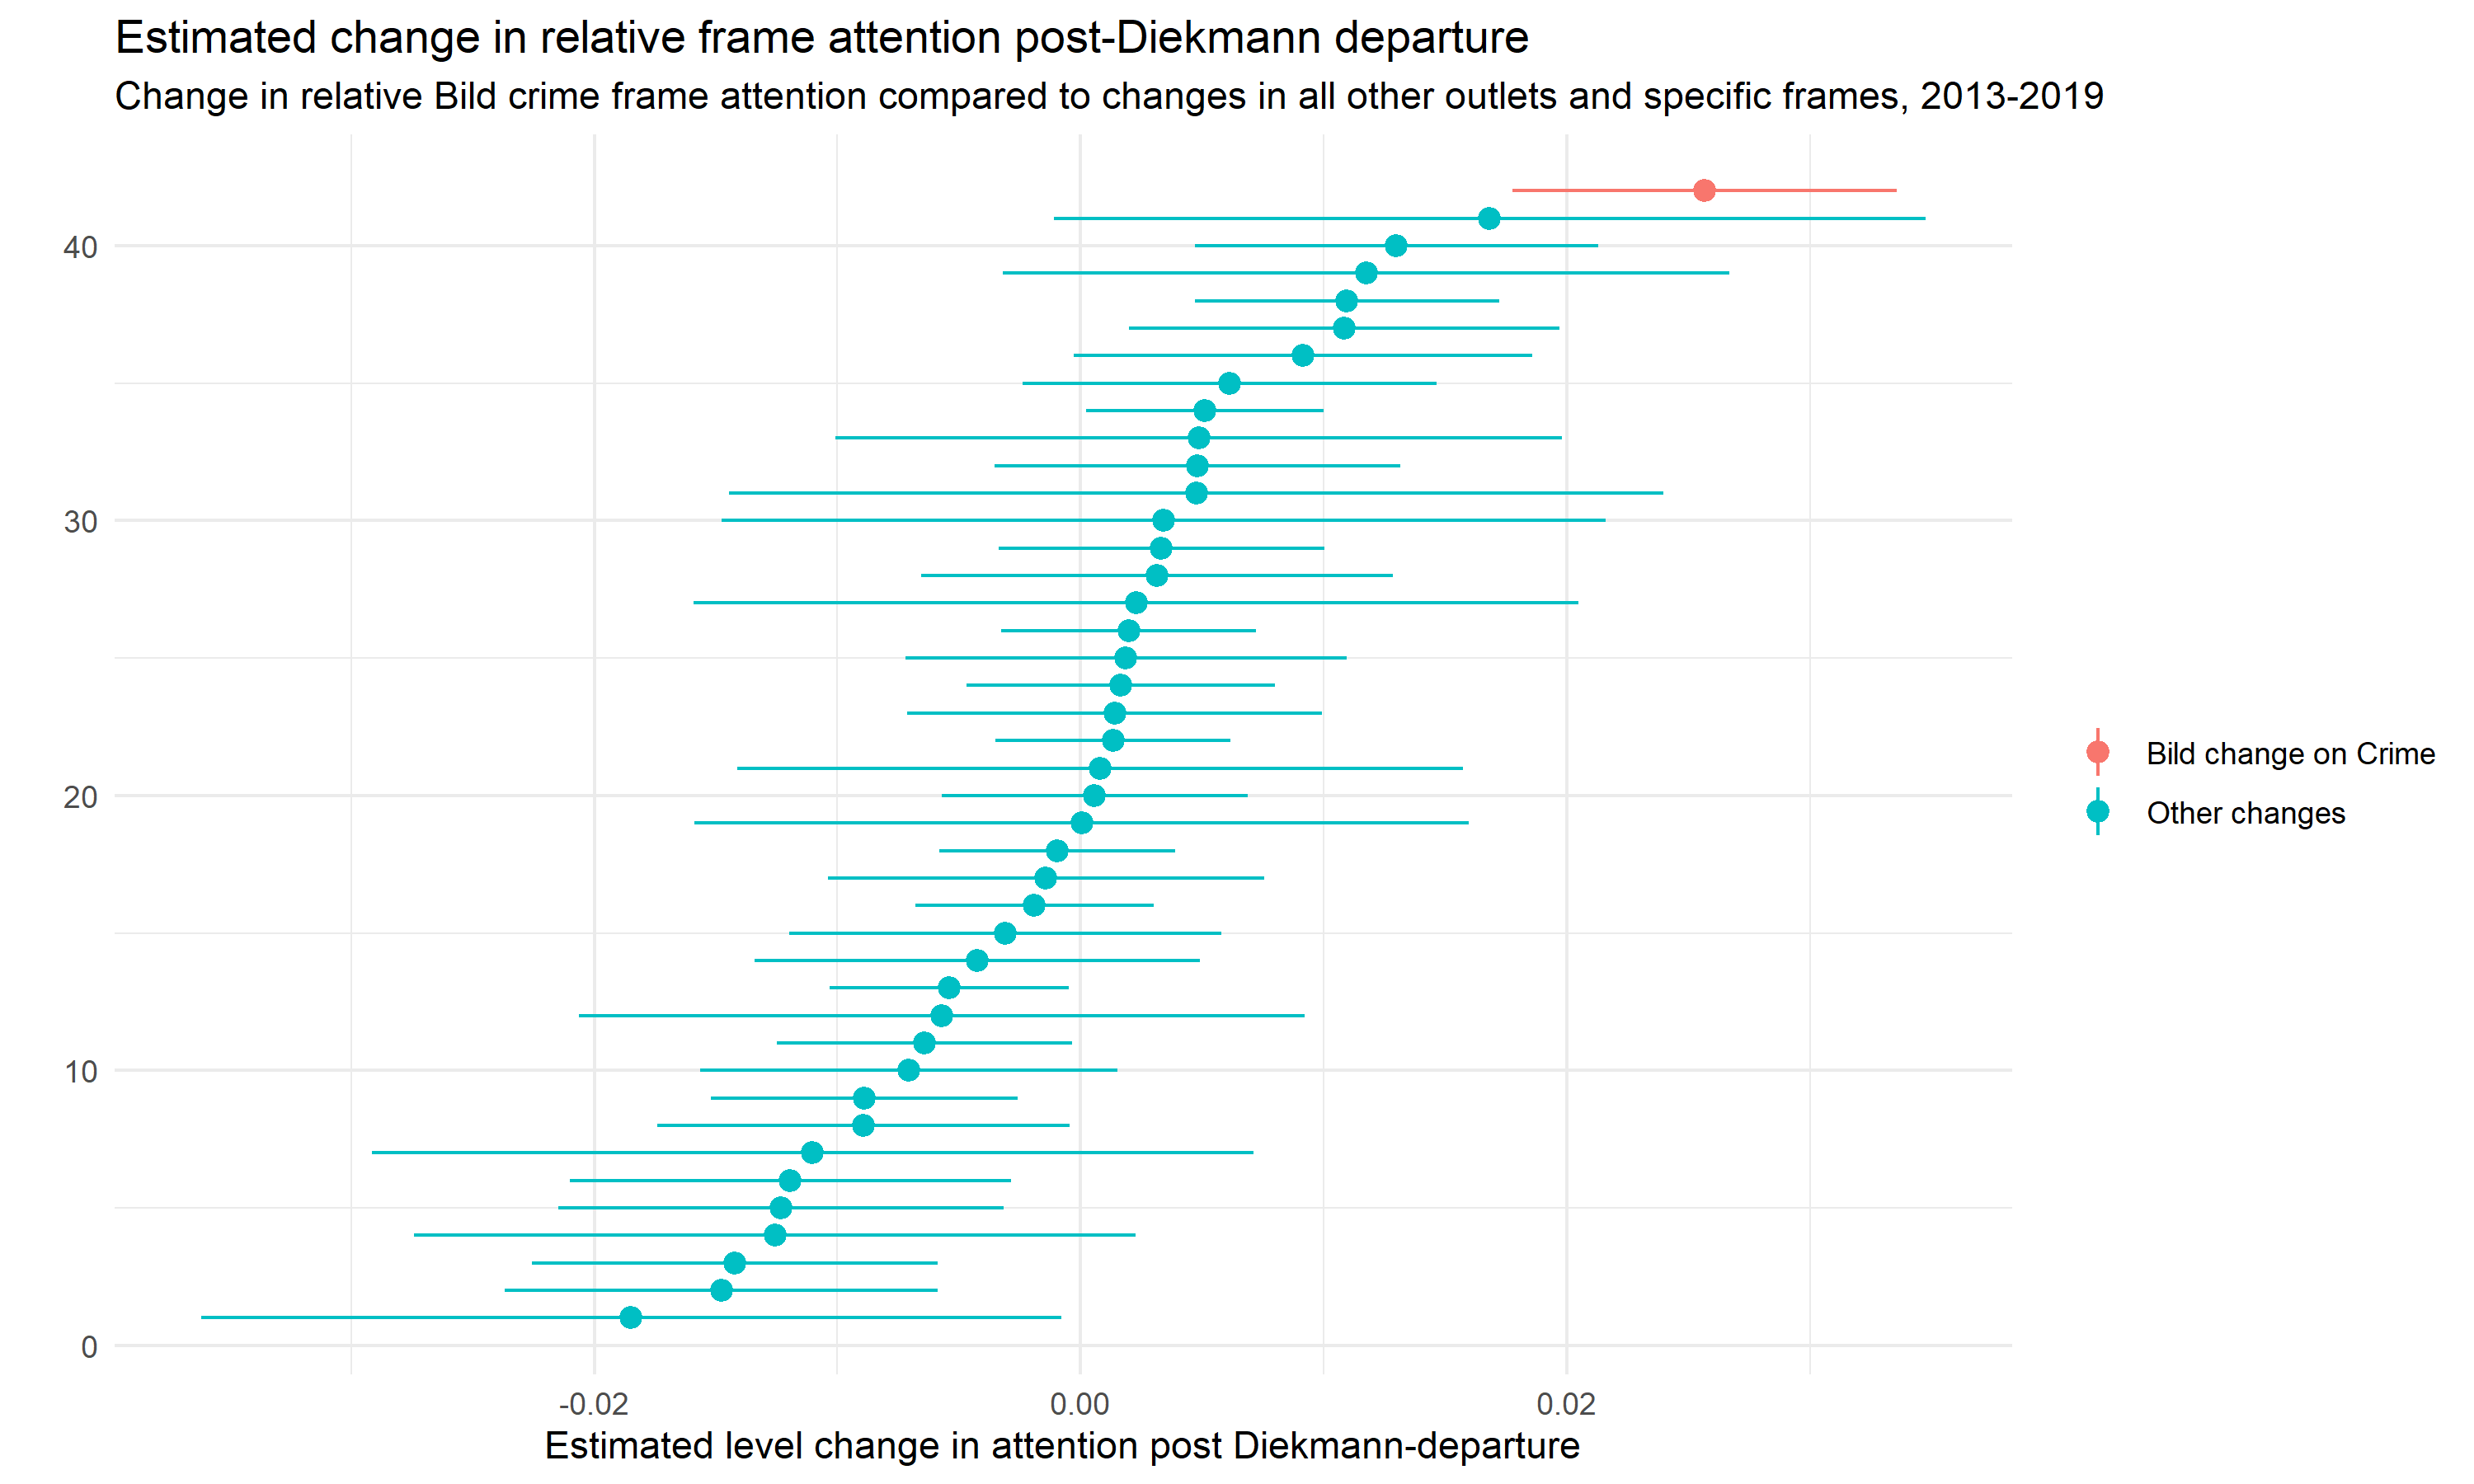
\includegraphics[width=\textwidth]{paper/vis/did_papers_frames_all_scatter.png}
\end{figure}

\begin{figure}[!ht]
    \centering
    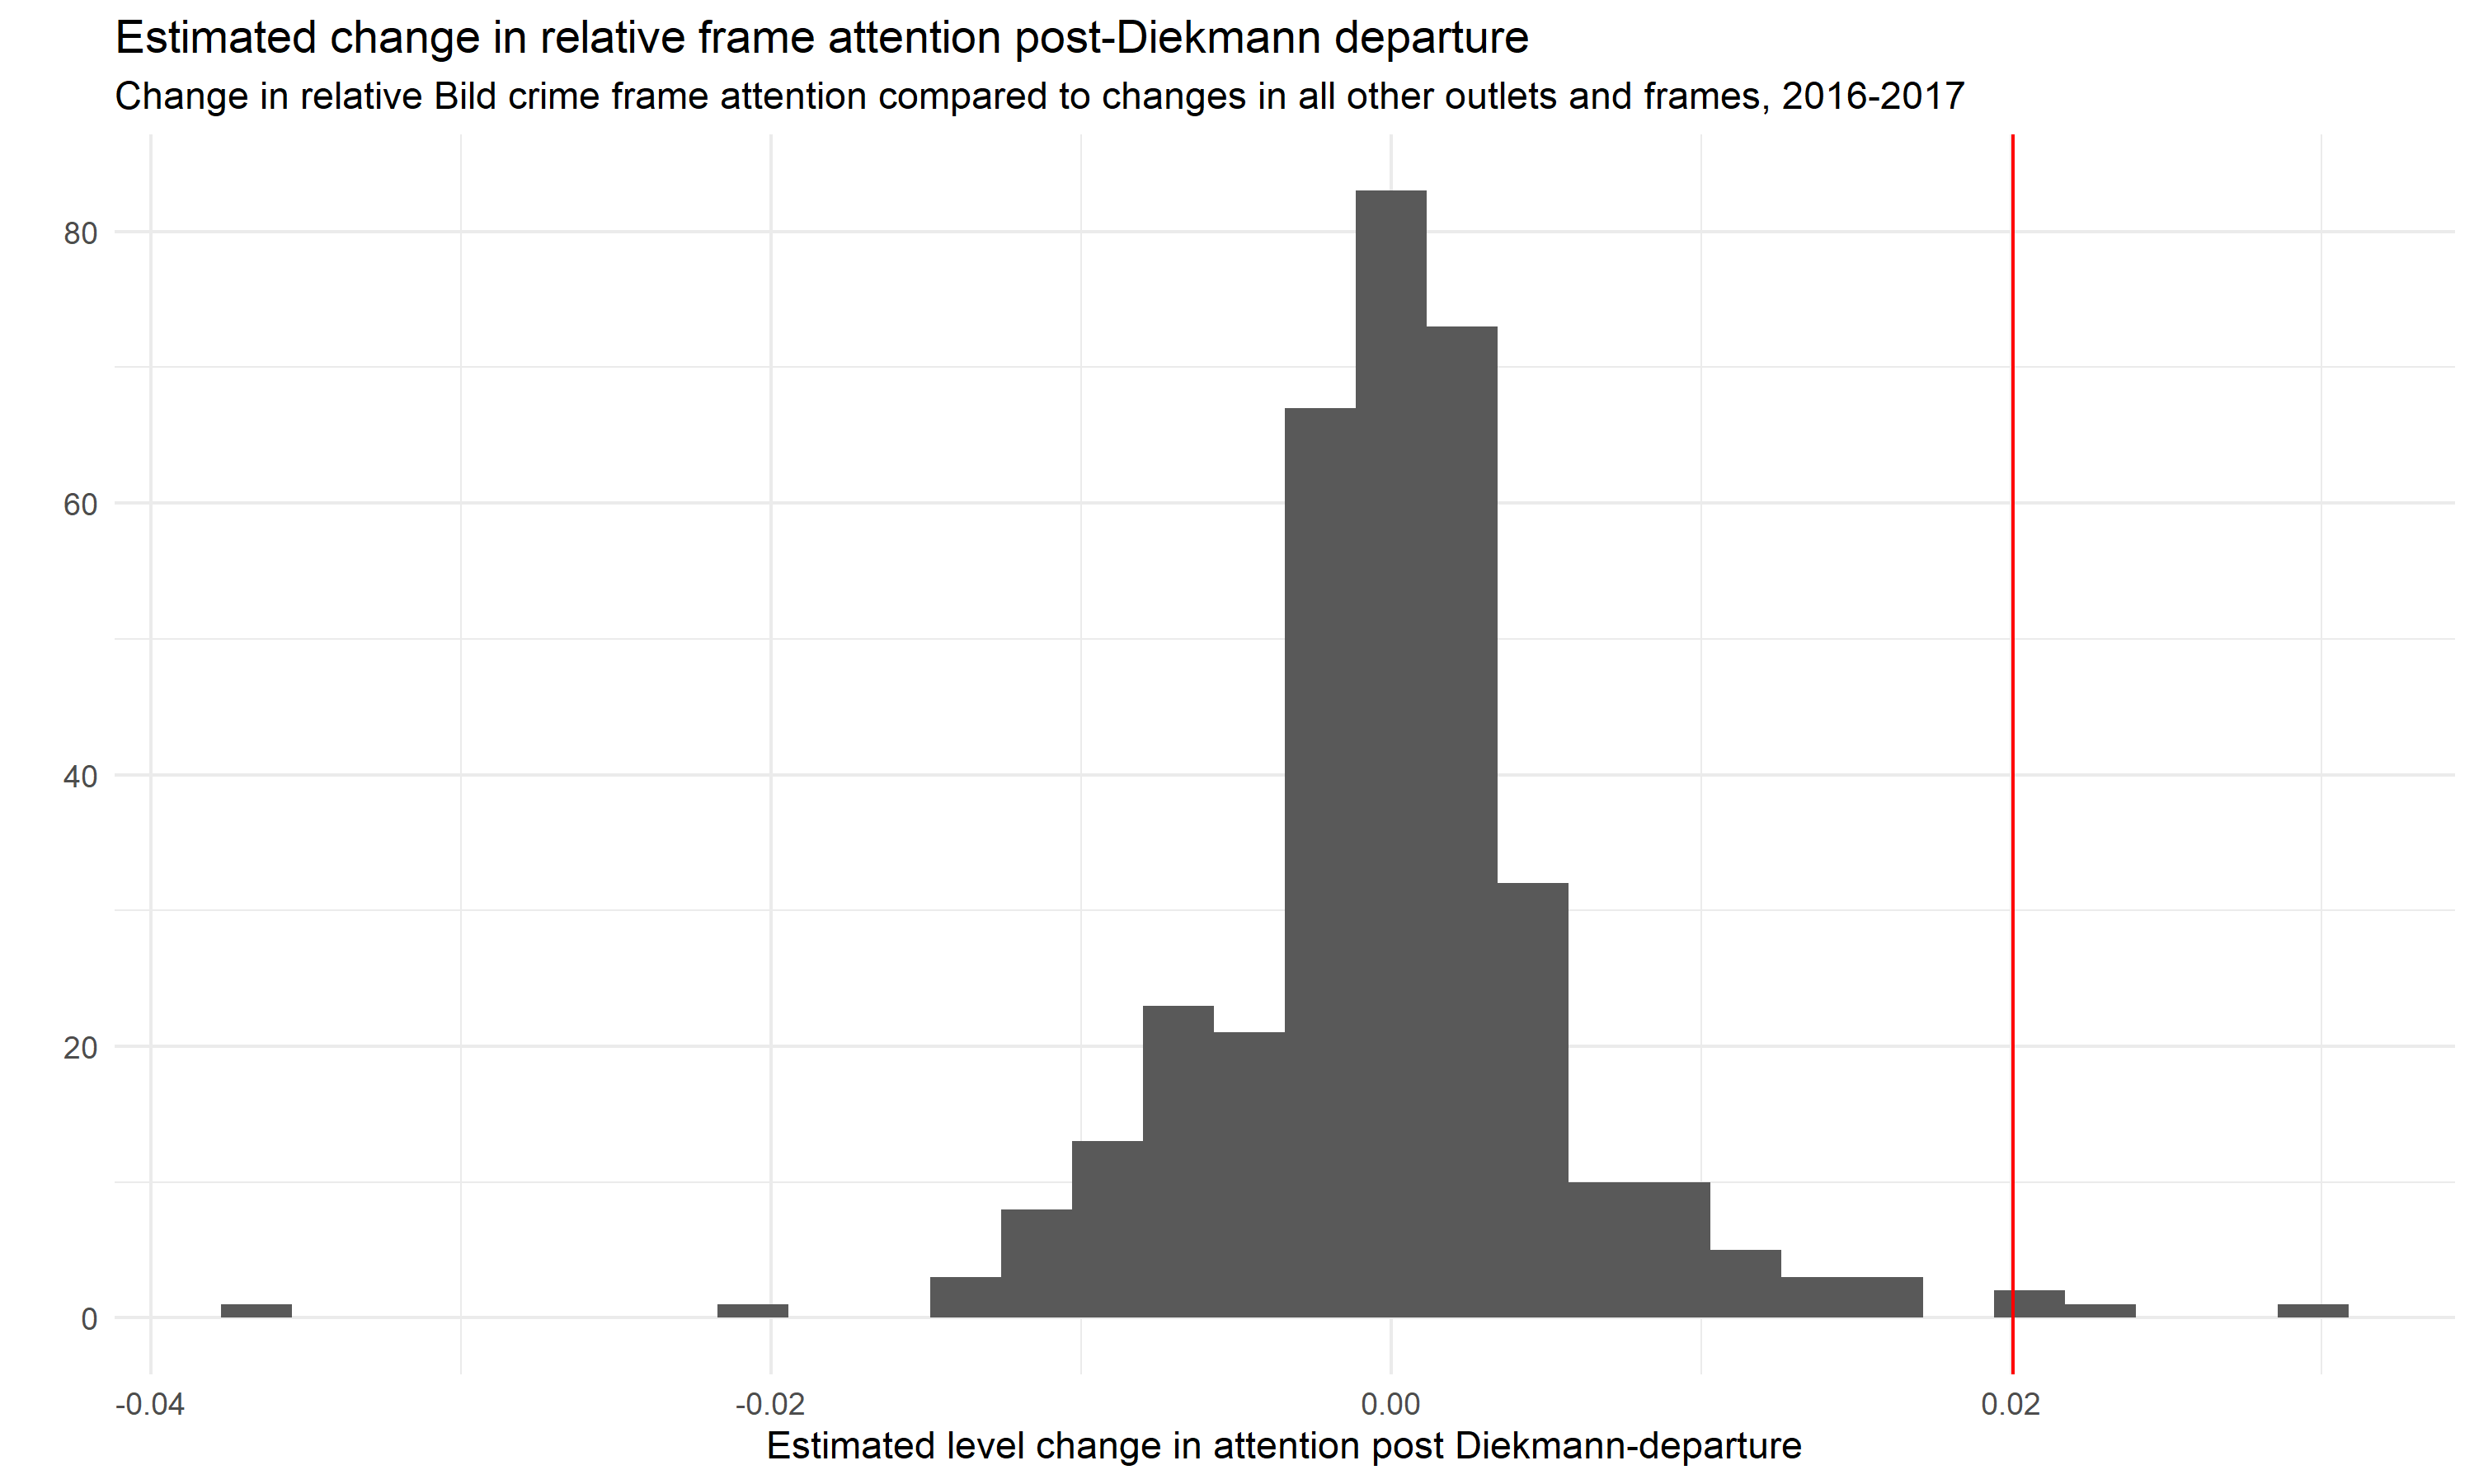
\includegraphics[width=\textwidth]{paper/vis/did_papers_allframes_1617_hist.png}
\end{figure}

\newpage

\subsection{DiD-assumption: Parallel trends}\label{sec:did_ass}


DiD-designs rest on the assumption that treated and untreated units would follow the same trend, were it not for the treatment. This means that, generally, treated and untreated units should show similar trends. Returning to figure \ref{fig:issues}, we can safely state that the parallel trends assumption is met in this case. All reader groups move in a highly similar fashion on both variables, albeit at different levels, which reflect the ideological leaning of their newspaper.

\subsection{Distribution of DiD-effect significance}\label{sec:did_sig}

\begin{figure}[!ht]
    \centering
    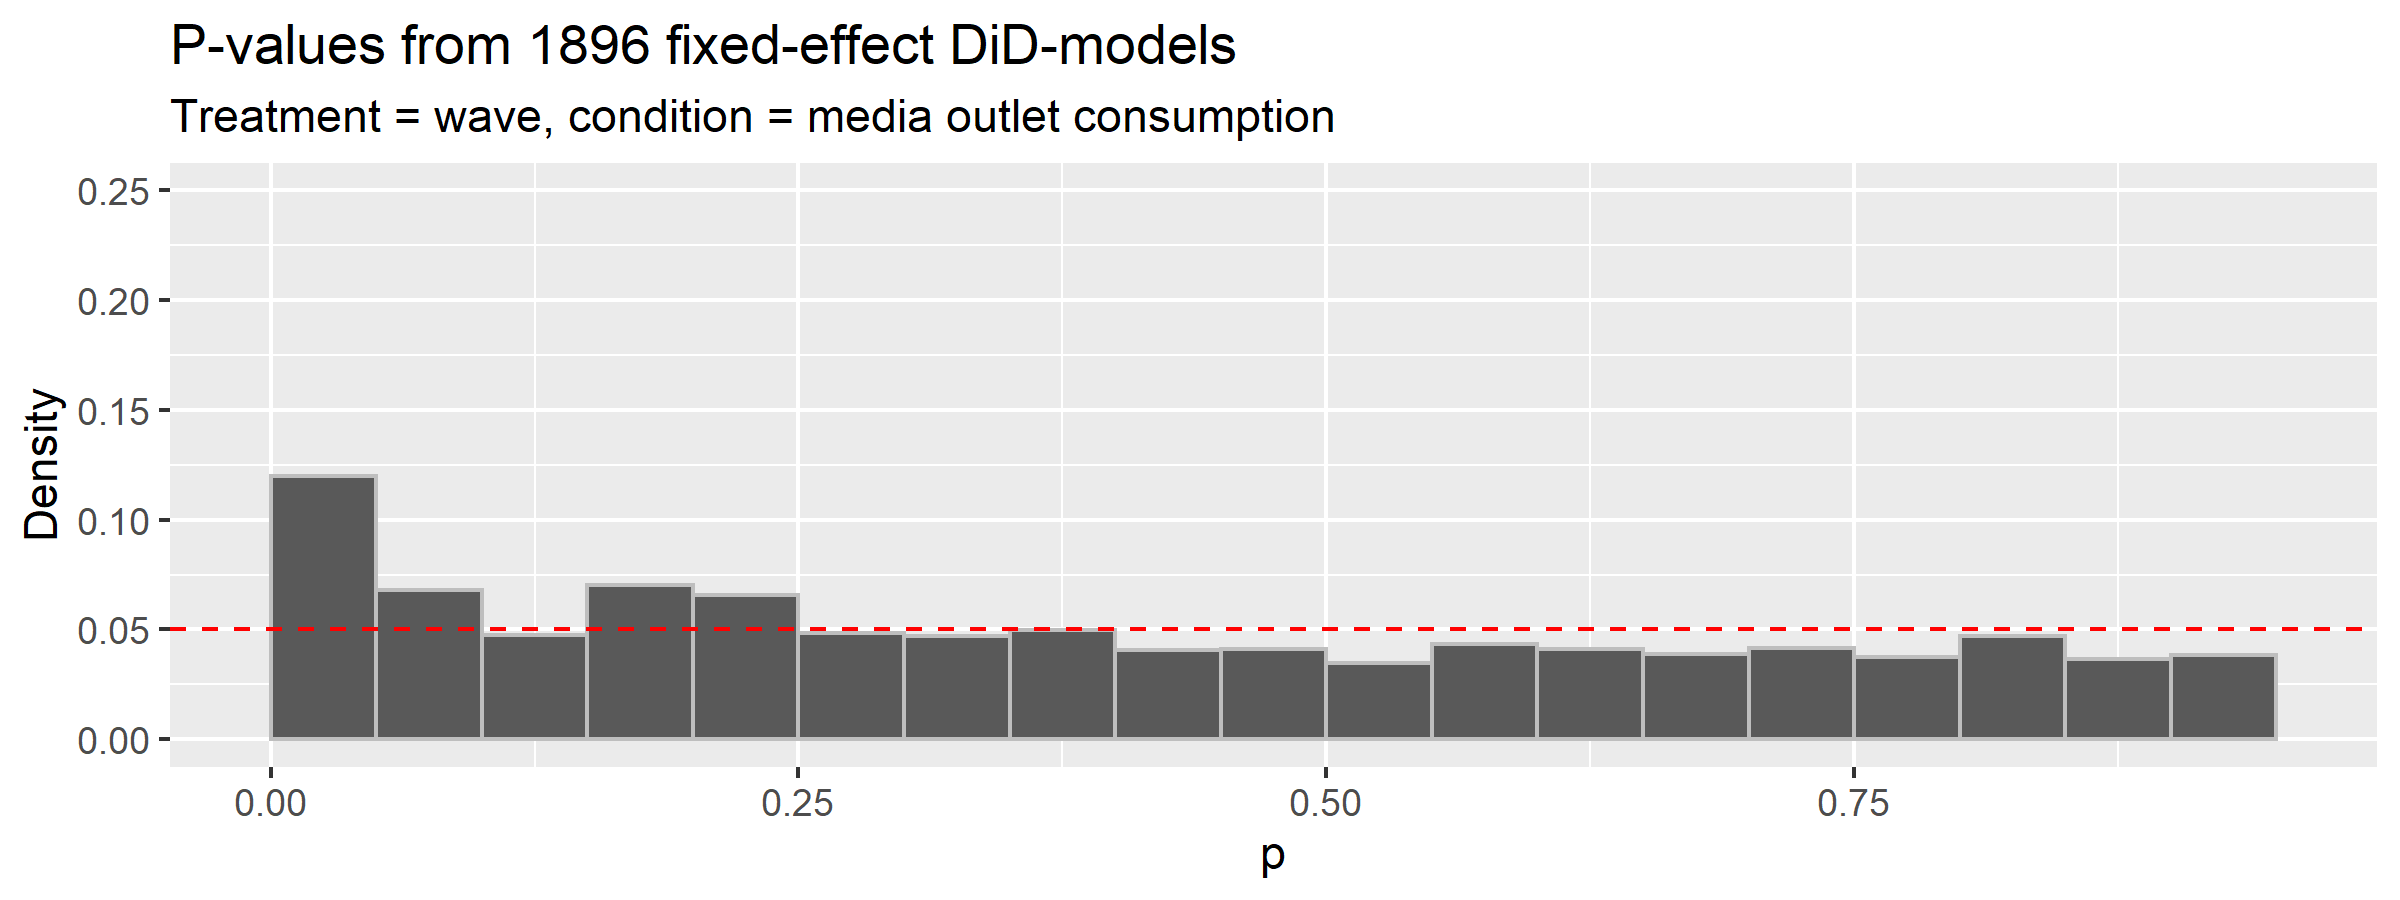
\includegraphics[width=\textwidth]{paper/vis/DiD_model_ps_notheory.png}
    \caption{P-values of 1,752 DiD-models estimating attitudinal shifts of media consumers, relative to consumers of other outlets.}
    \label{fig:p_values}
\end{figure}

These highly parallel trends might raise another problem, however. Possibly, no significant variation of reader groups' migration opinion from the general trend can be observed. To address this concern, I estimate DiDs for all wave-issue-paper combinations. This means I use attitudinal questions on all political issues included in the GLES Panel (economic, issues, climate, ...), and assess whether news consumption matters for opinion formation more generally. Figure \ref{fig:p_values} shows the distribution of p-values for the DiD-term from 1,752 fixed-effect models with GLES Panel data. The distribution shows a considerable deviation from the expected uniform distribution (red line) were there no explaining variation in the DiD-term beyond the uniform effects of wave and paper readership. This means, more often than random (12\% vs 5\%), the opinions of consumers of certain news deviate from the opinions of other citizens. This is even more severe for the 192 wave-paper combinations concerning the immigration or integration item used in the remainder of this study, where 18\% of all estimated DiDs fall under the 5\%-threshold\footnote{See plot \ref{fig:p-val_imm}}.  This strongly indicates that news consumption matters for opinion formation and that the data shows variation which can be explained, despite highly parallel trends.

\begin{figure}[!ht]
    \centering
    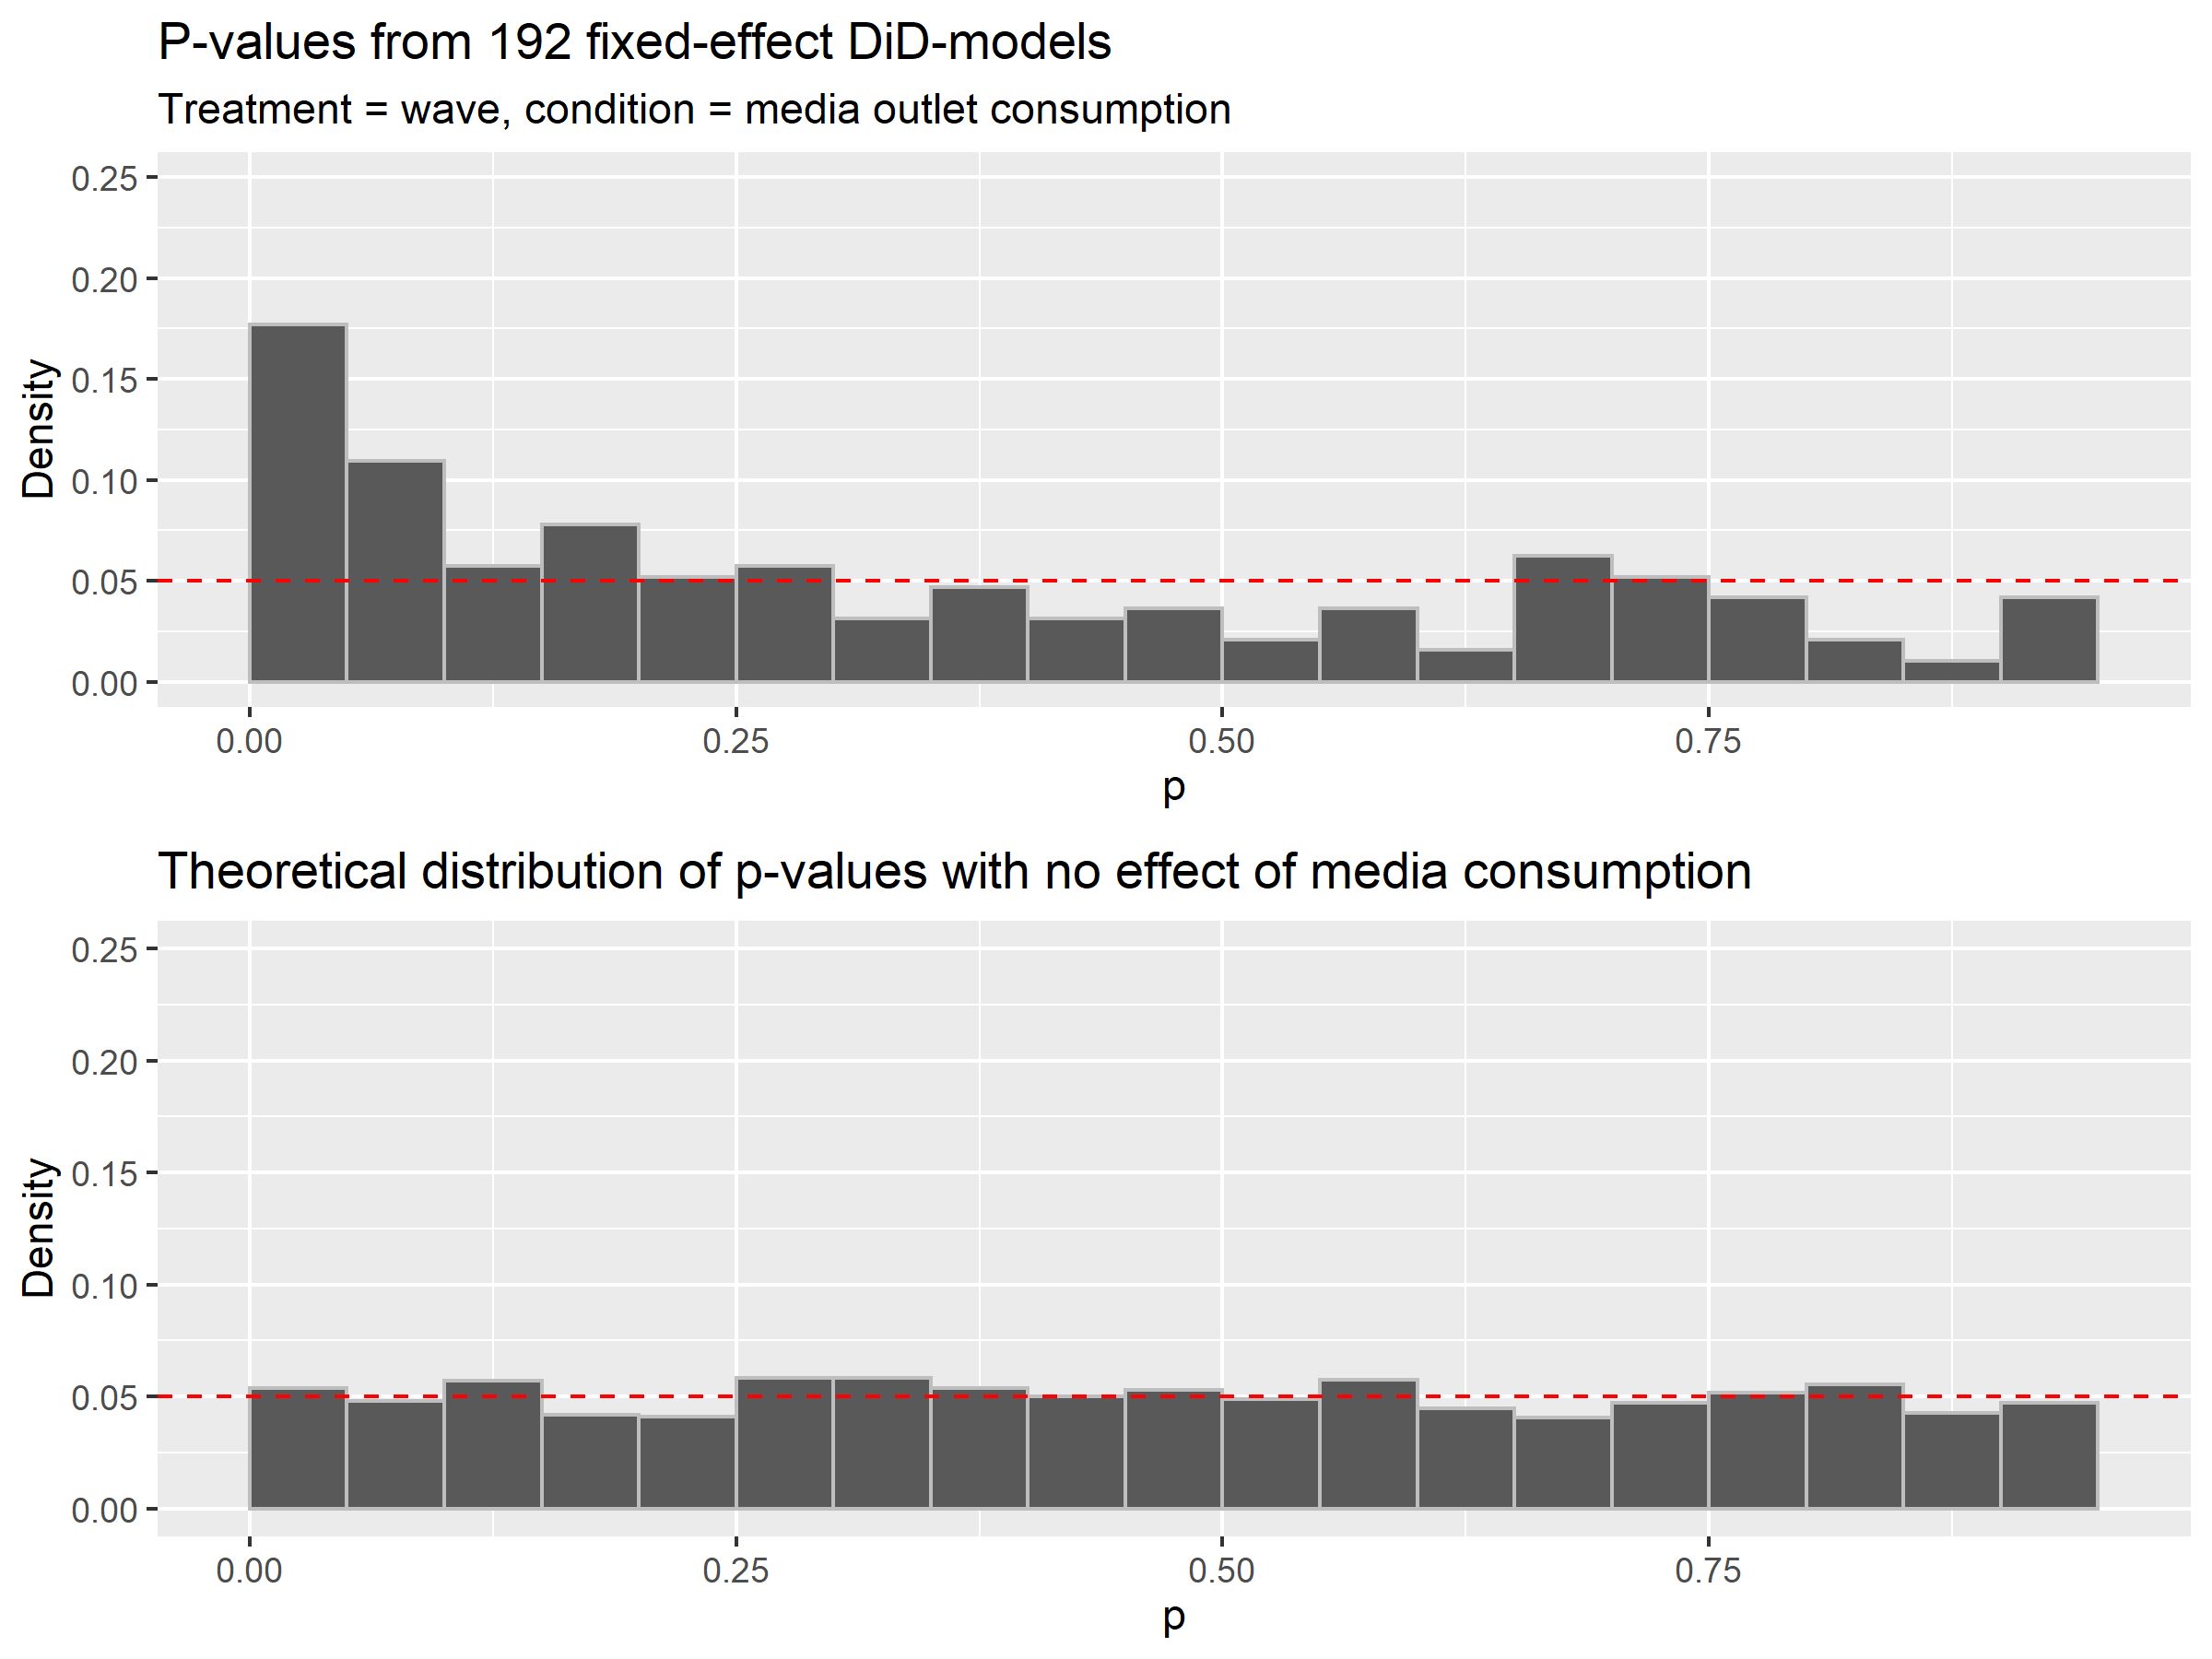
\includegraphics[width=\textwidth]{paper/vis/DiD_model_ps_immint.png}
    \caption{Empirical and theoretical p-values of 192 DiD-models corresponding to the immigration and integration questions of the GLES.}
    \label{fig:p-val_imm}
\end{figure}


\subsection{Opinion change among all and exclusive newspaper consumers}

\begin{figure}
    \centering
    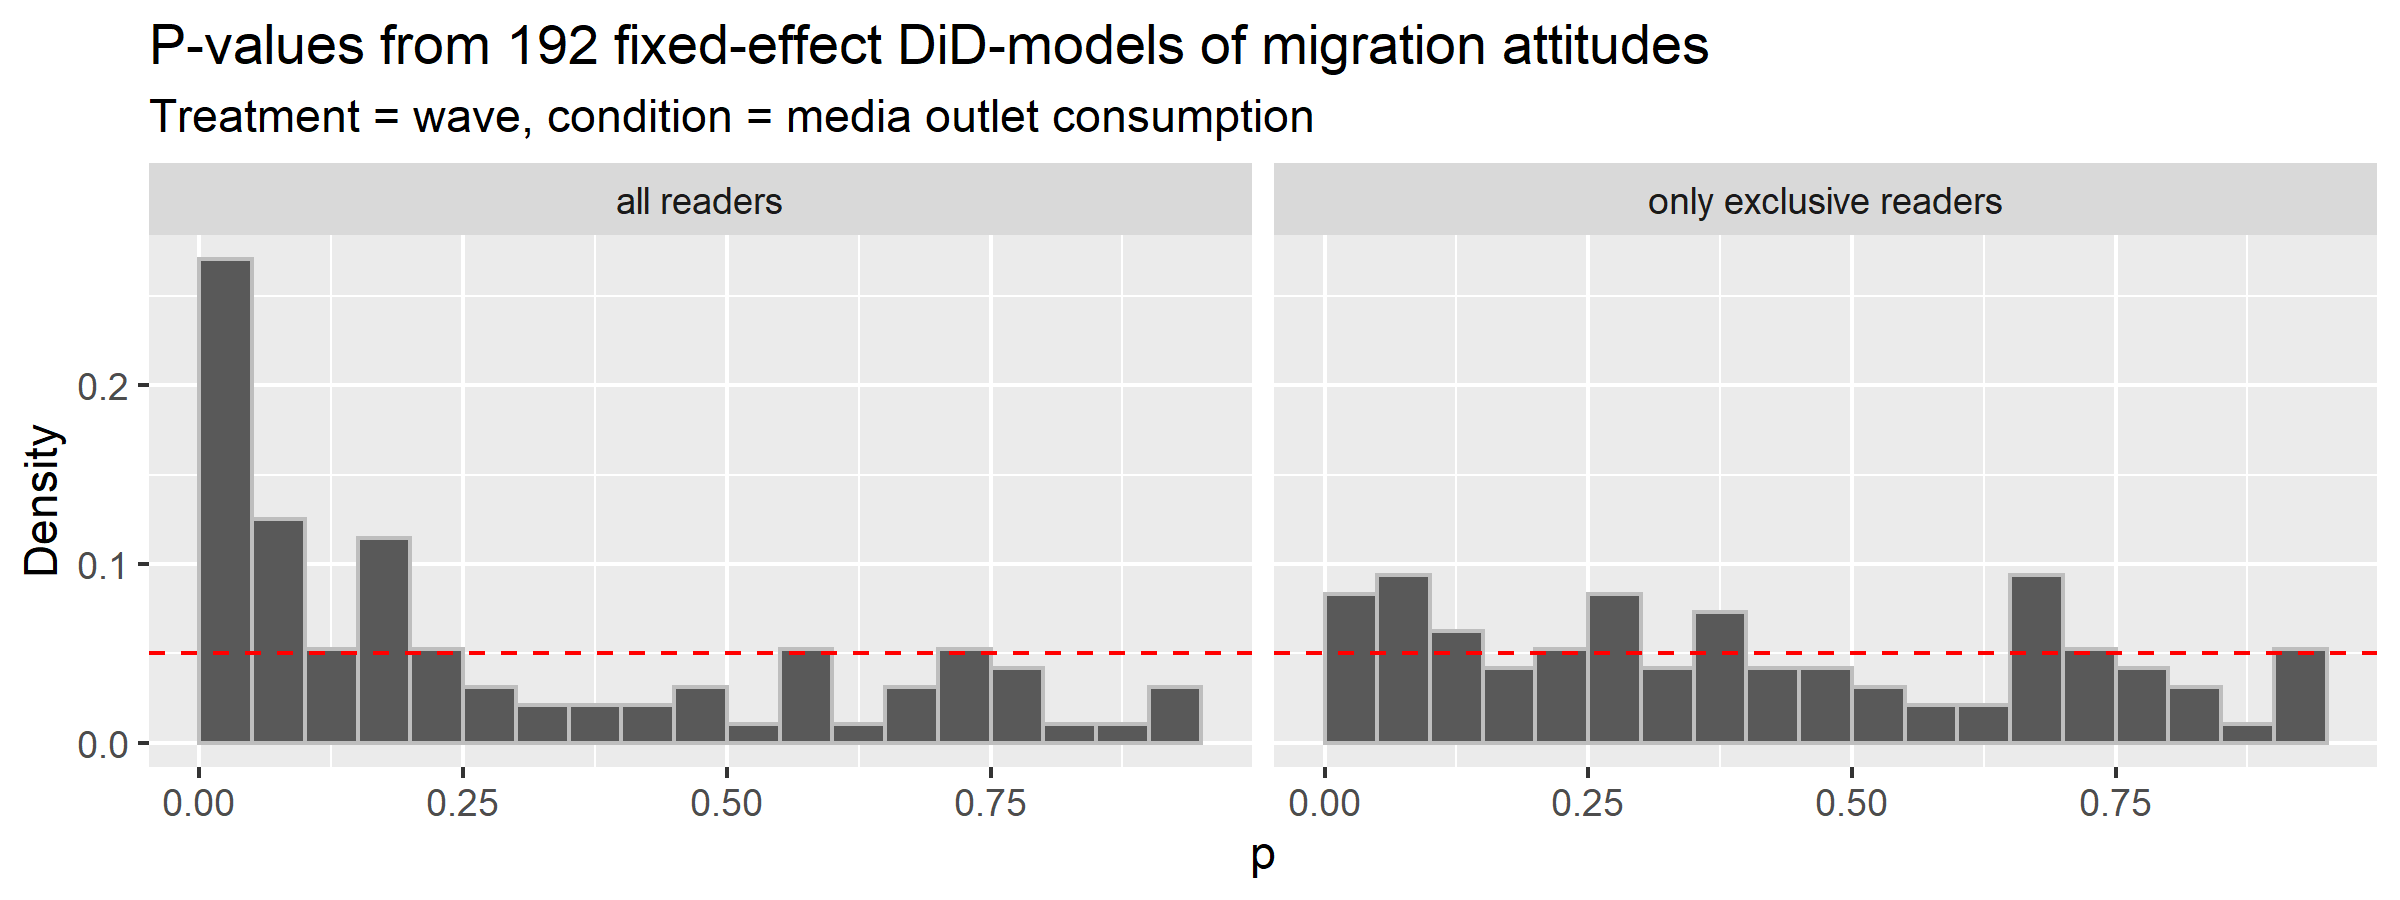
\includegraphics[width=\textwidth]{paper/vis/DiD_model_ps_immint_bytreat.png}
    \caption{Empirical p-values of 192 DiD-models showing opinion change for different treatment definitions.}
    \label{fig:did_by_treat}
\end{figure}

\end{document}

\subsection{Extended migration dictionary}\label{app:dictionary}

The extended migration dictionary for the pre-sampling of articles on migration consists of 35 terms (matching both lower and upper case): \textit{asyl, asylant, asylanten, asylbewerber, asylbewerberin, auslander, einwanderer, einwandernde, einwanderung, migration, immigration, schutzsuchende, visa, visum, zuwanderung, zuwanderer, zuwandernde, ausländer, ausländerinnen, flüchtling, flüchtende, flüchtlinge, flüchtlingen, migranten, vertriebene, asylantinnen, asylbewerberinnen, auslanderinnen, einwandererin, einwandererinnen, fluchtling, fluchtende, fluchtlinge, schutzbedurftige, schutzbedürftige.}

\newpage

\subsection{Structural Topic Model}\label{app:stm}

\begin{figure}[!ht]
    \centering
    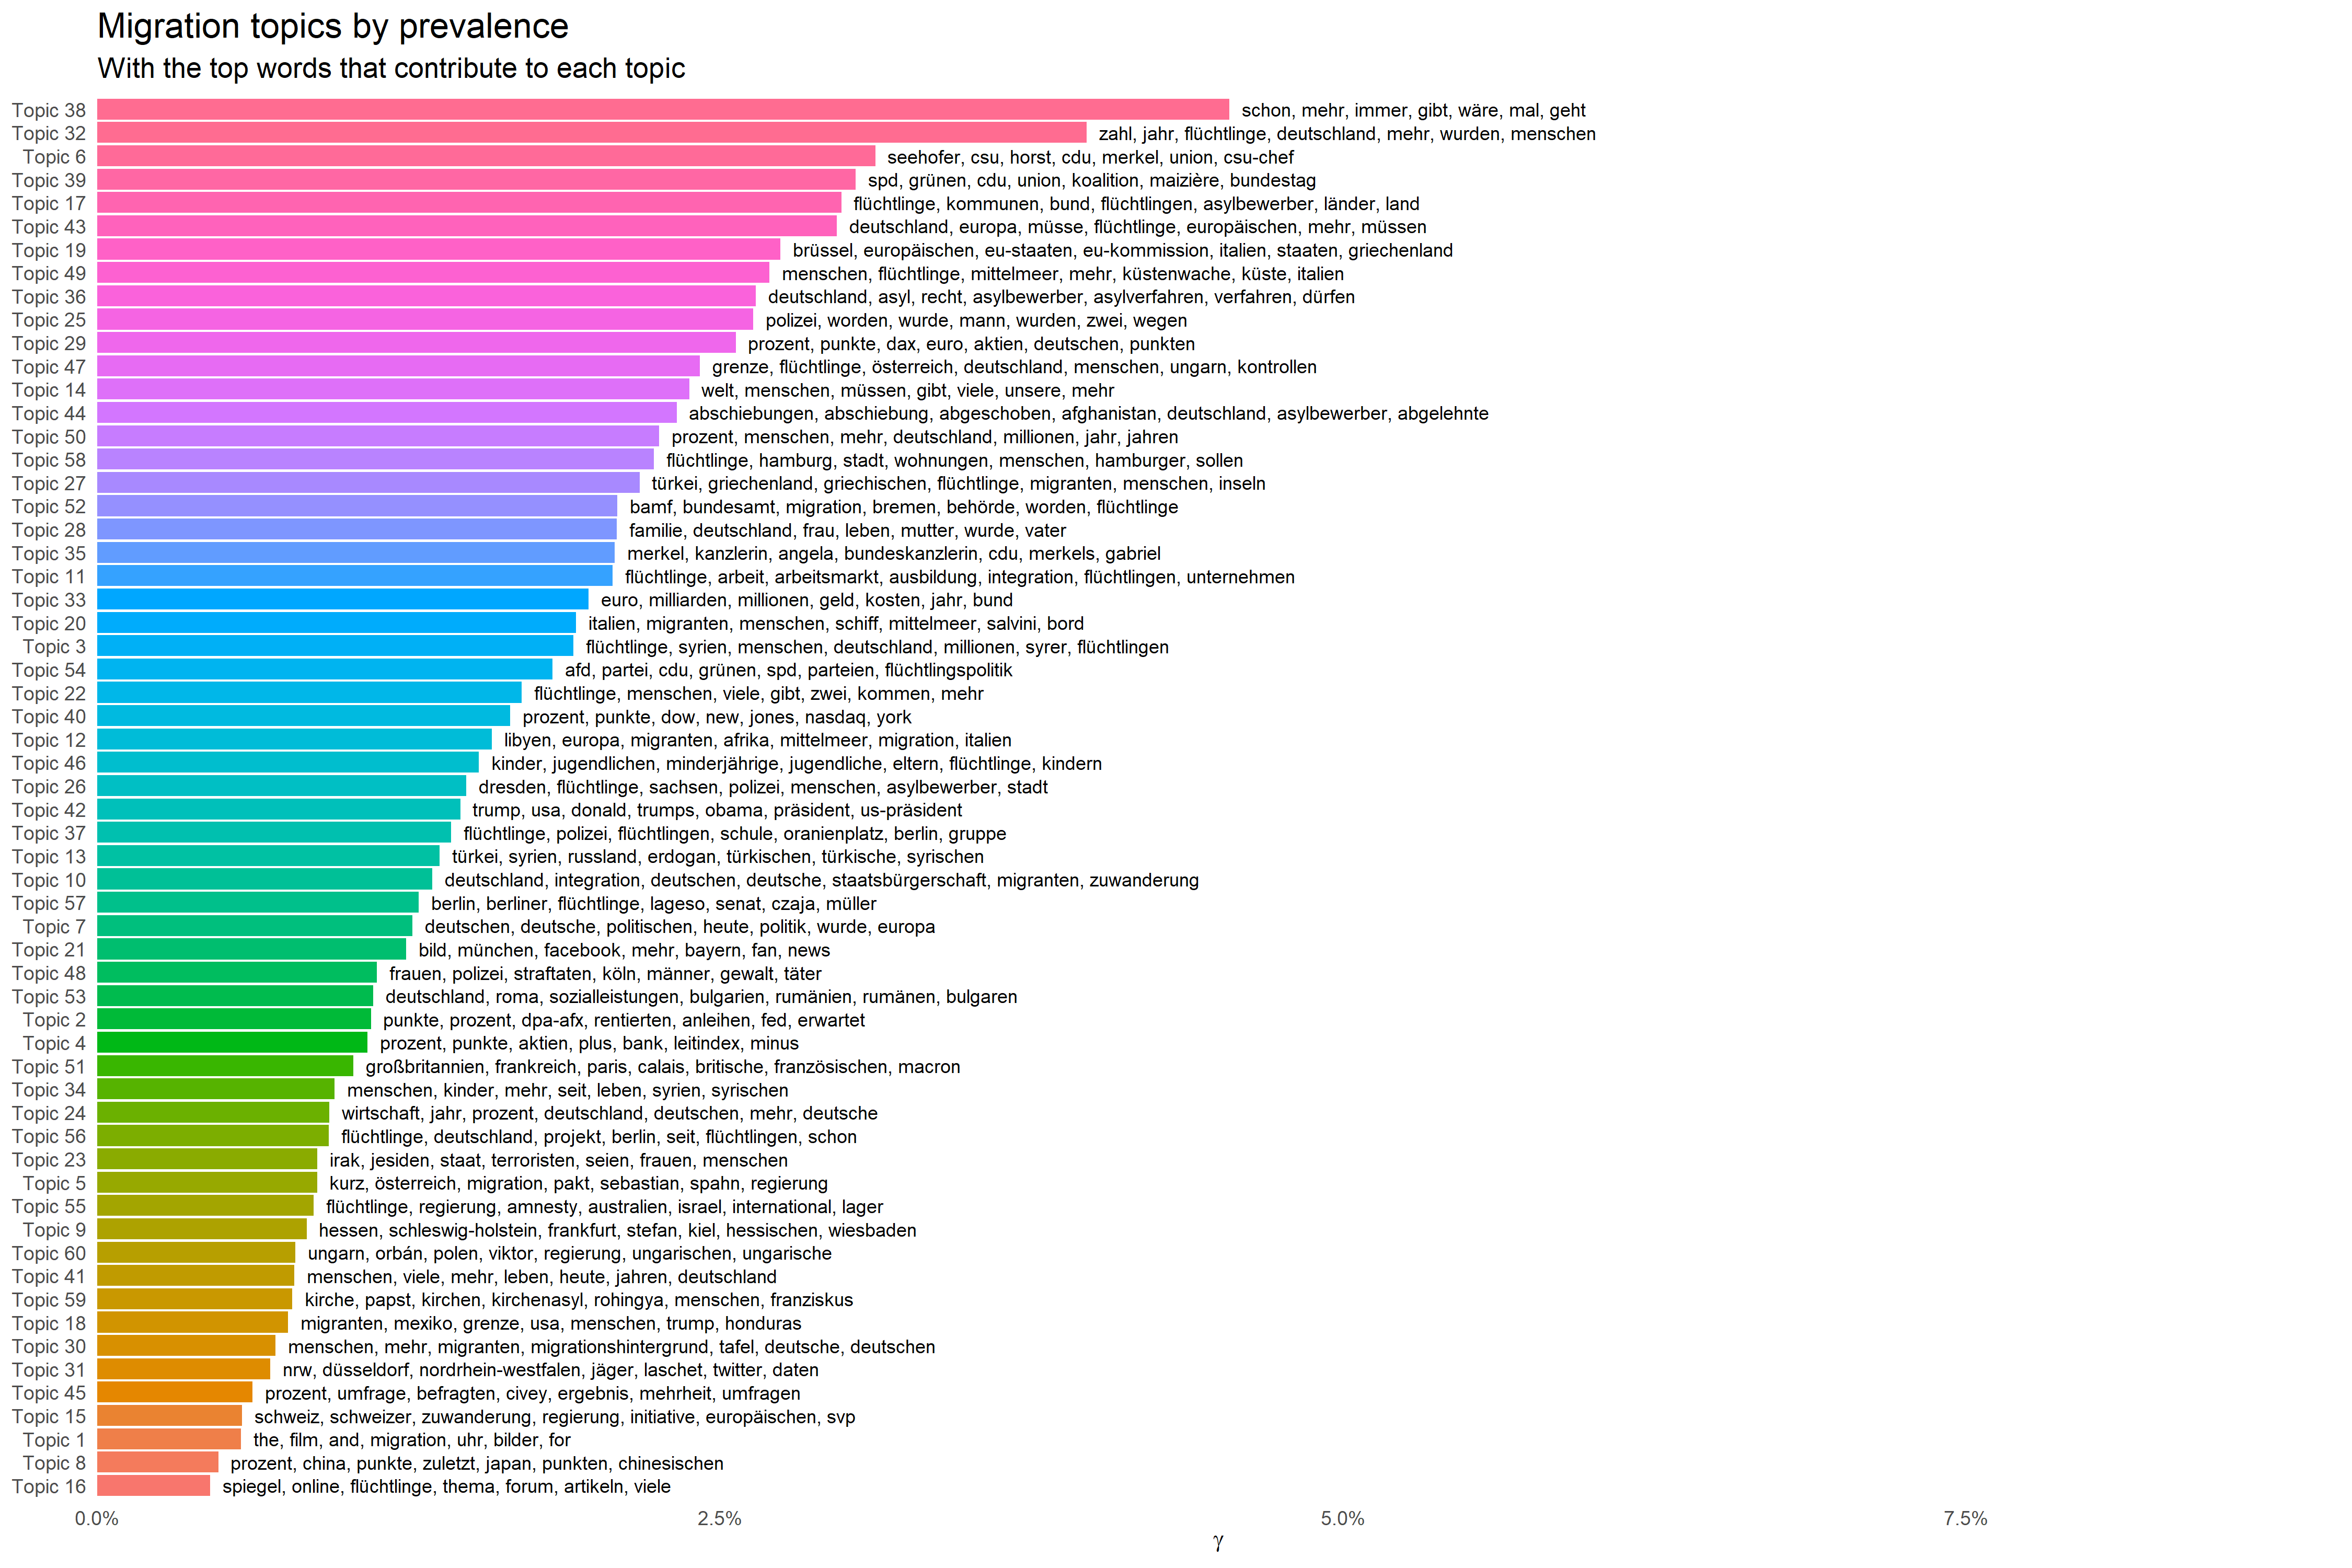
\includegraphics[width=2\textwidth]{paper/vis/mig_topics_plot.png}
    \label{fig:topics}
\end{figure}

\newpage

